% !TEX root = ./../main.tex
\chapter{Molecular description of the process}
%Introduzione a seguito dei risultati con la metadinamica: run unbiased con PW striped, random11, random 12 e POPC

\section{Water dragging}
%Trascinamento delle PW nelle varie salse

%	WPatchedComparison		WRPComparison
\begin{figure}[]
	\center
	\subfloat[striped – model comparison]{
		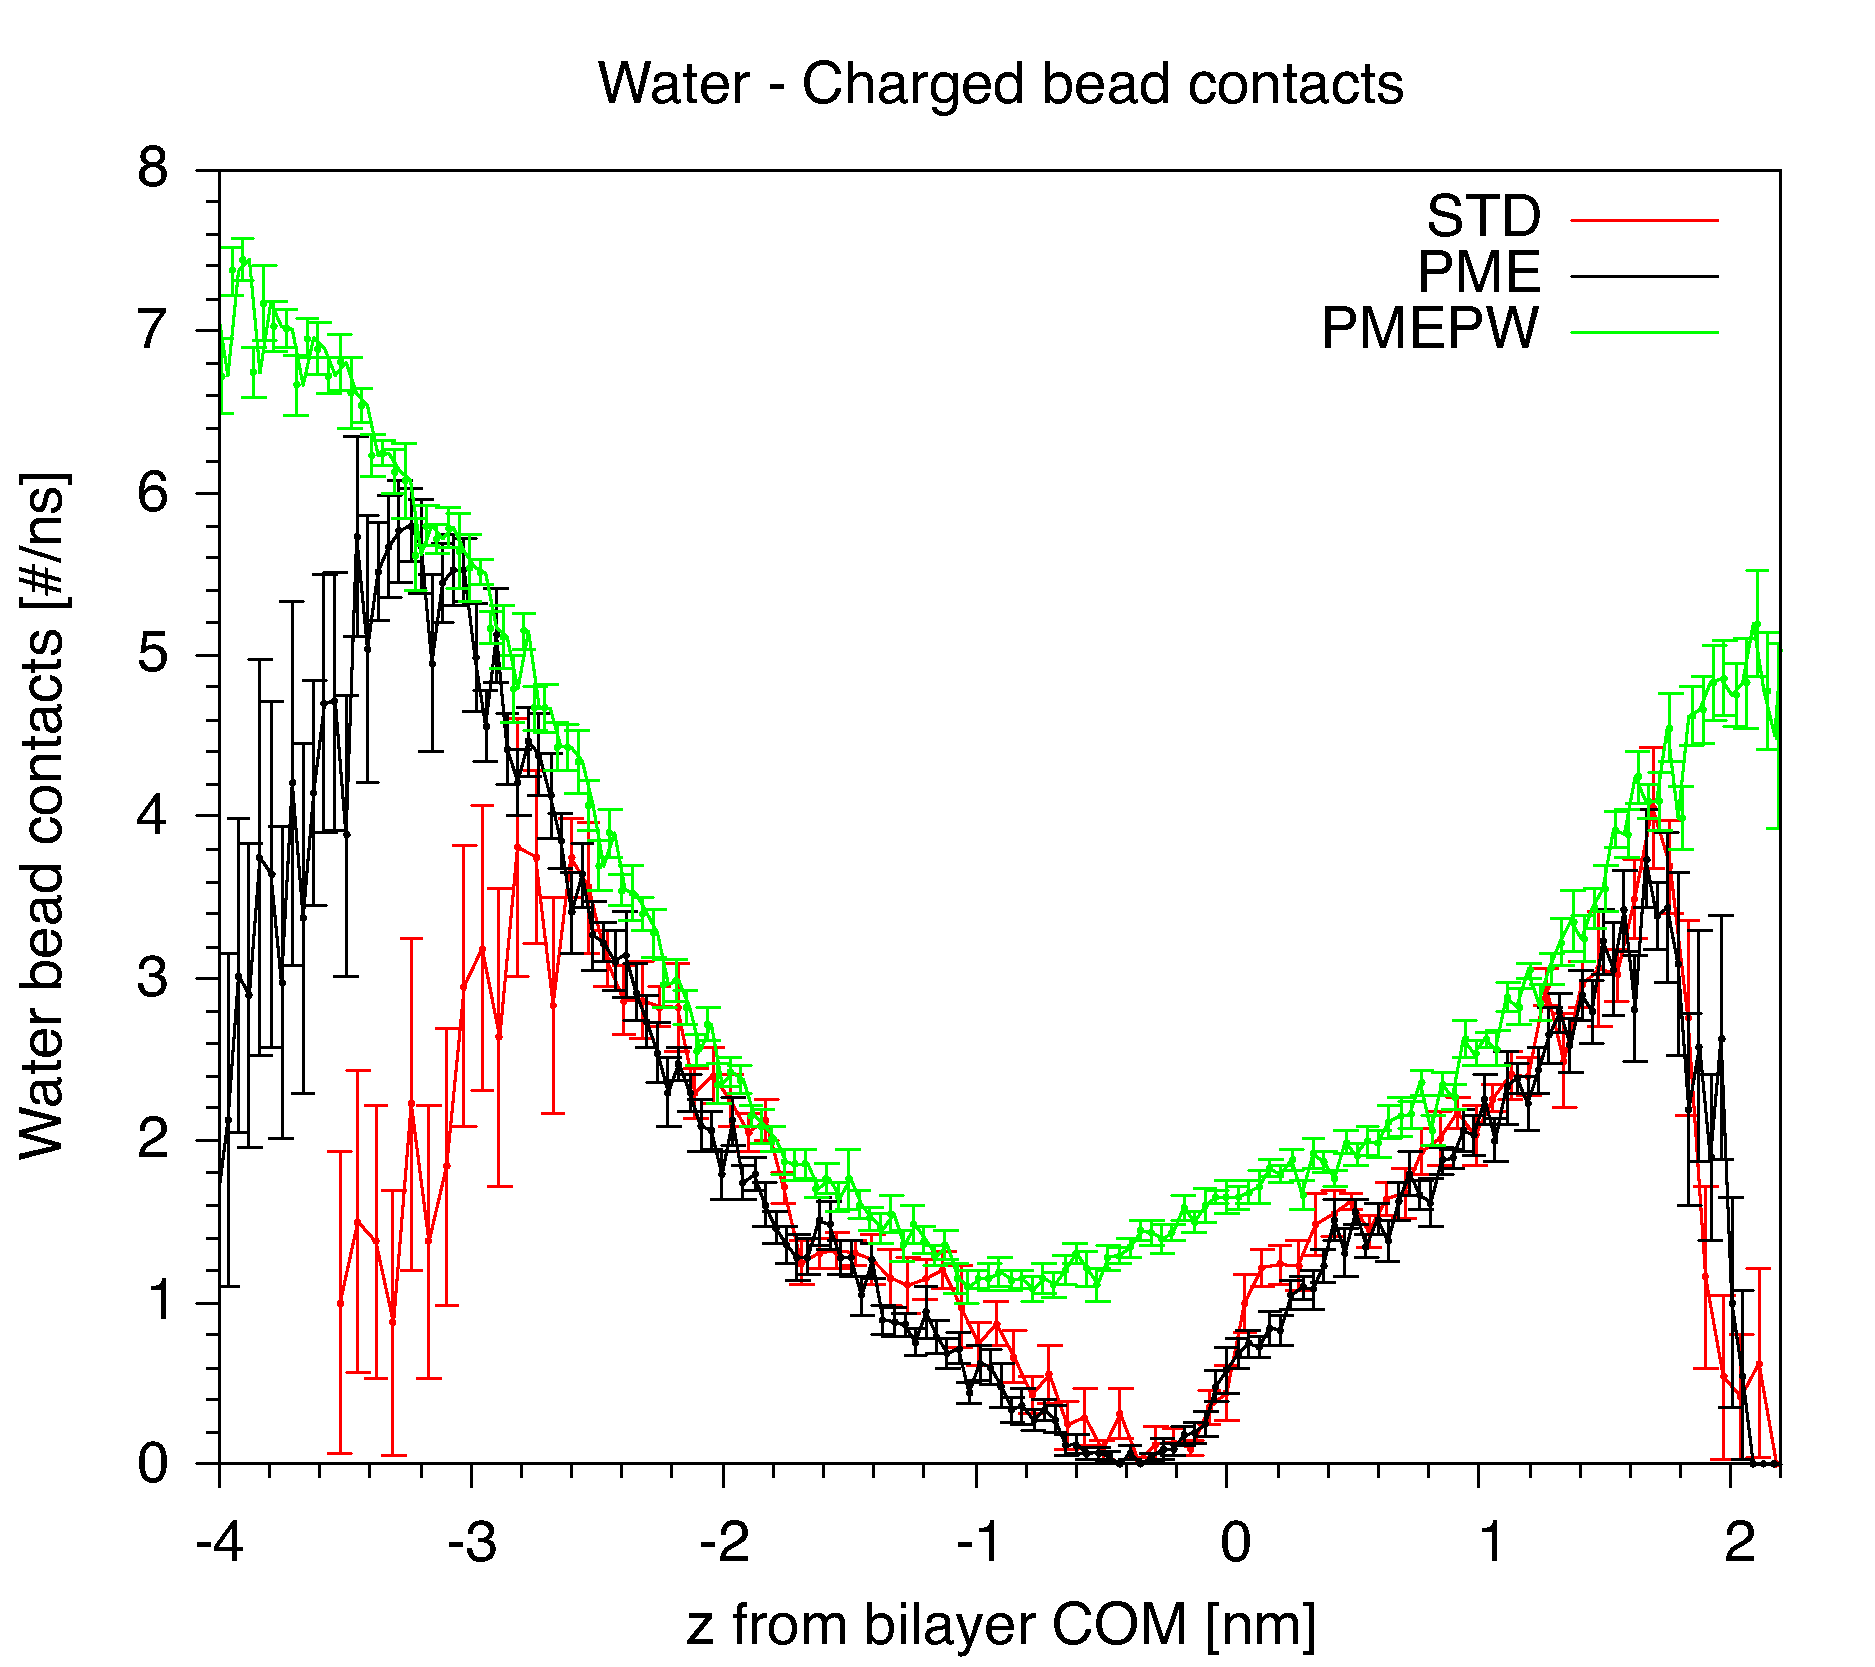
\includegraphics[width=0.5\textwidth]{./img/results/WPatchedComparison}
	}%
	\subfloat[striped – random comparison]{
		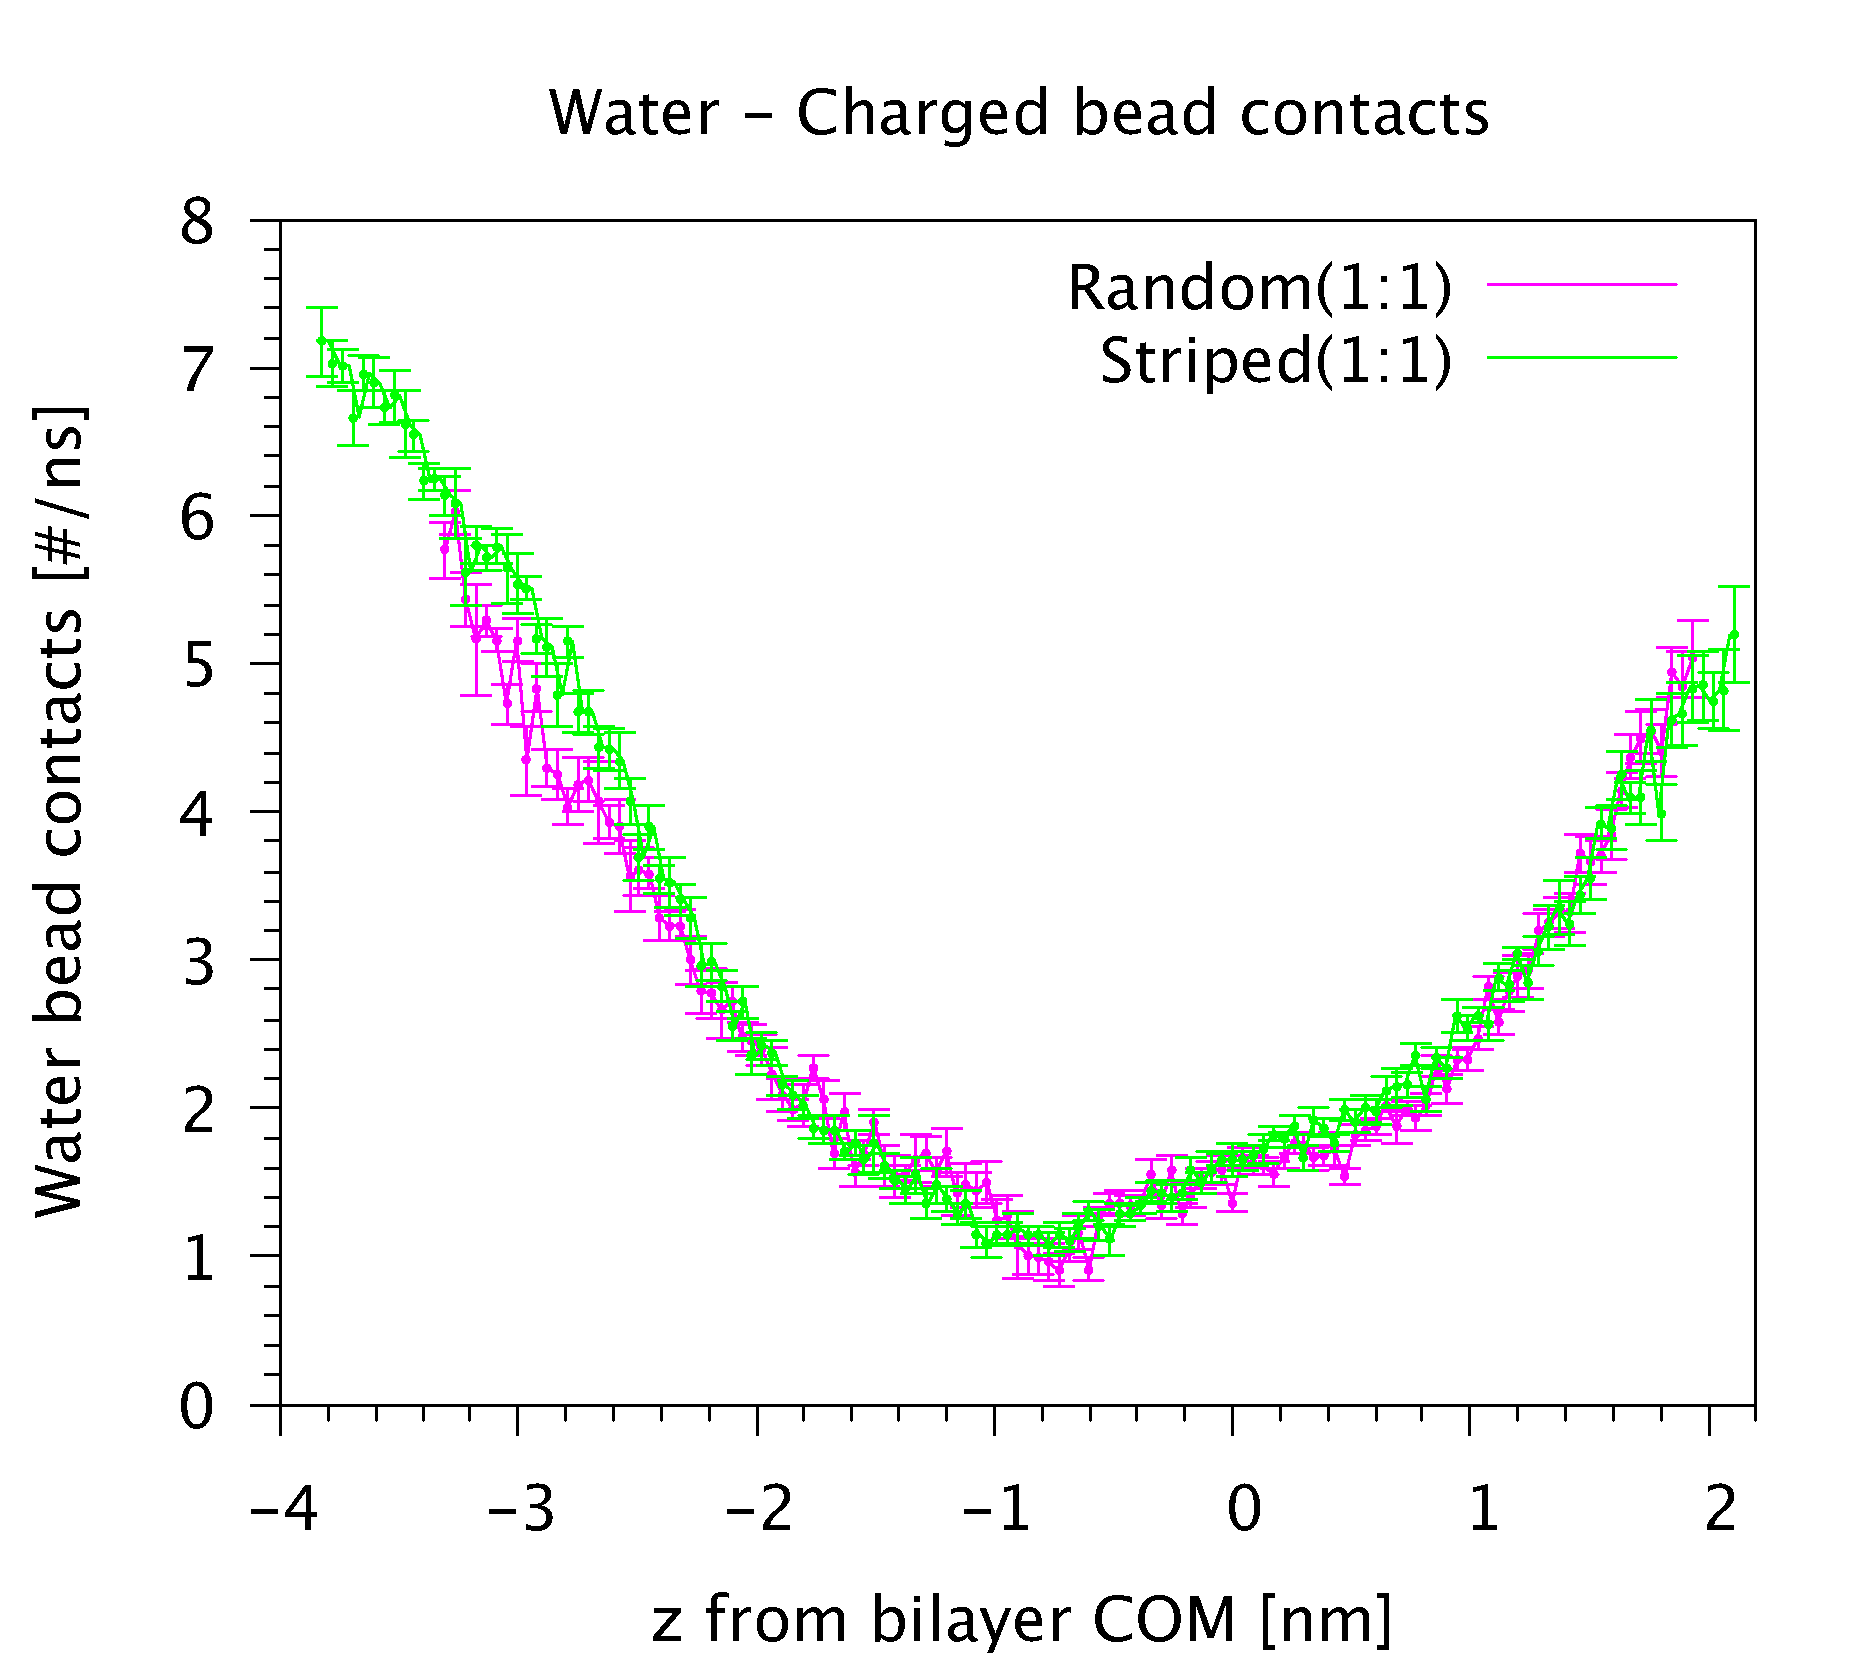
\includegraphics[width=0.5\textwidth]{./img/results/WRPComparison}
	}%
	\caption{Number of contacts per ns between water beads and the charged bead in function of the $z$ distance of the charged bead from the bilayer \acs{COM}. (a) For the striped \acs{NP} in comparison with different models. (b) In comparison between the striped and the random \acs{NP}s.}
\end{figure}


\section{Lipid heads dragging}
%Trascinamento delle teste dei lipidi nelle varie salse

% 	minDistPatched			minDistRandom11
\begin{figure}[p]
	\center
	\subfloat[striped NP]{
		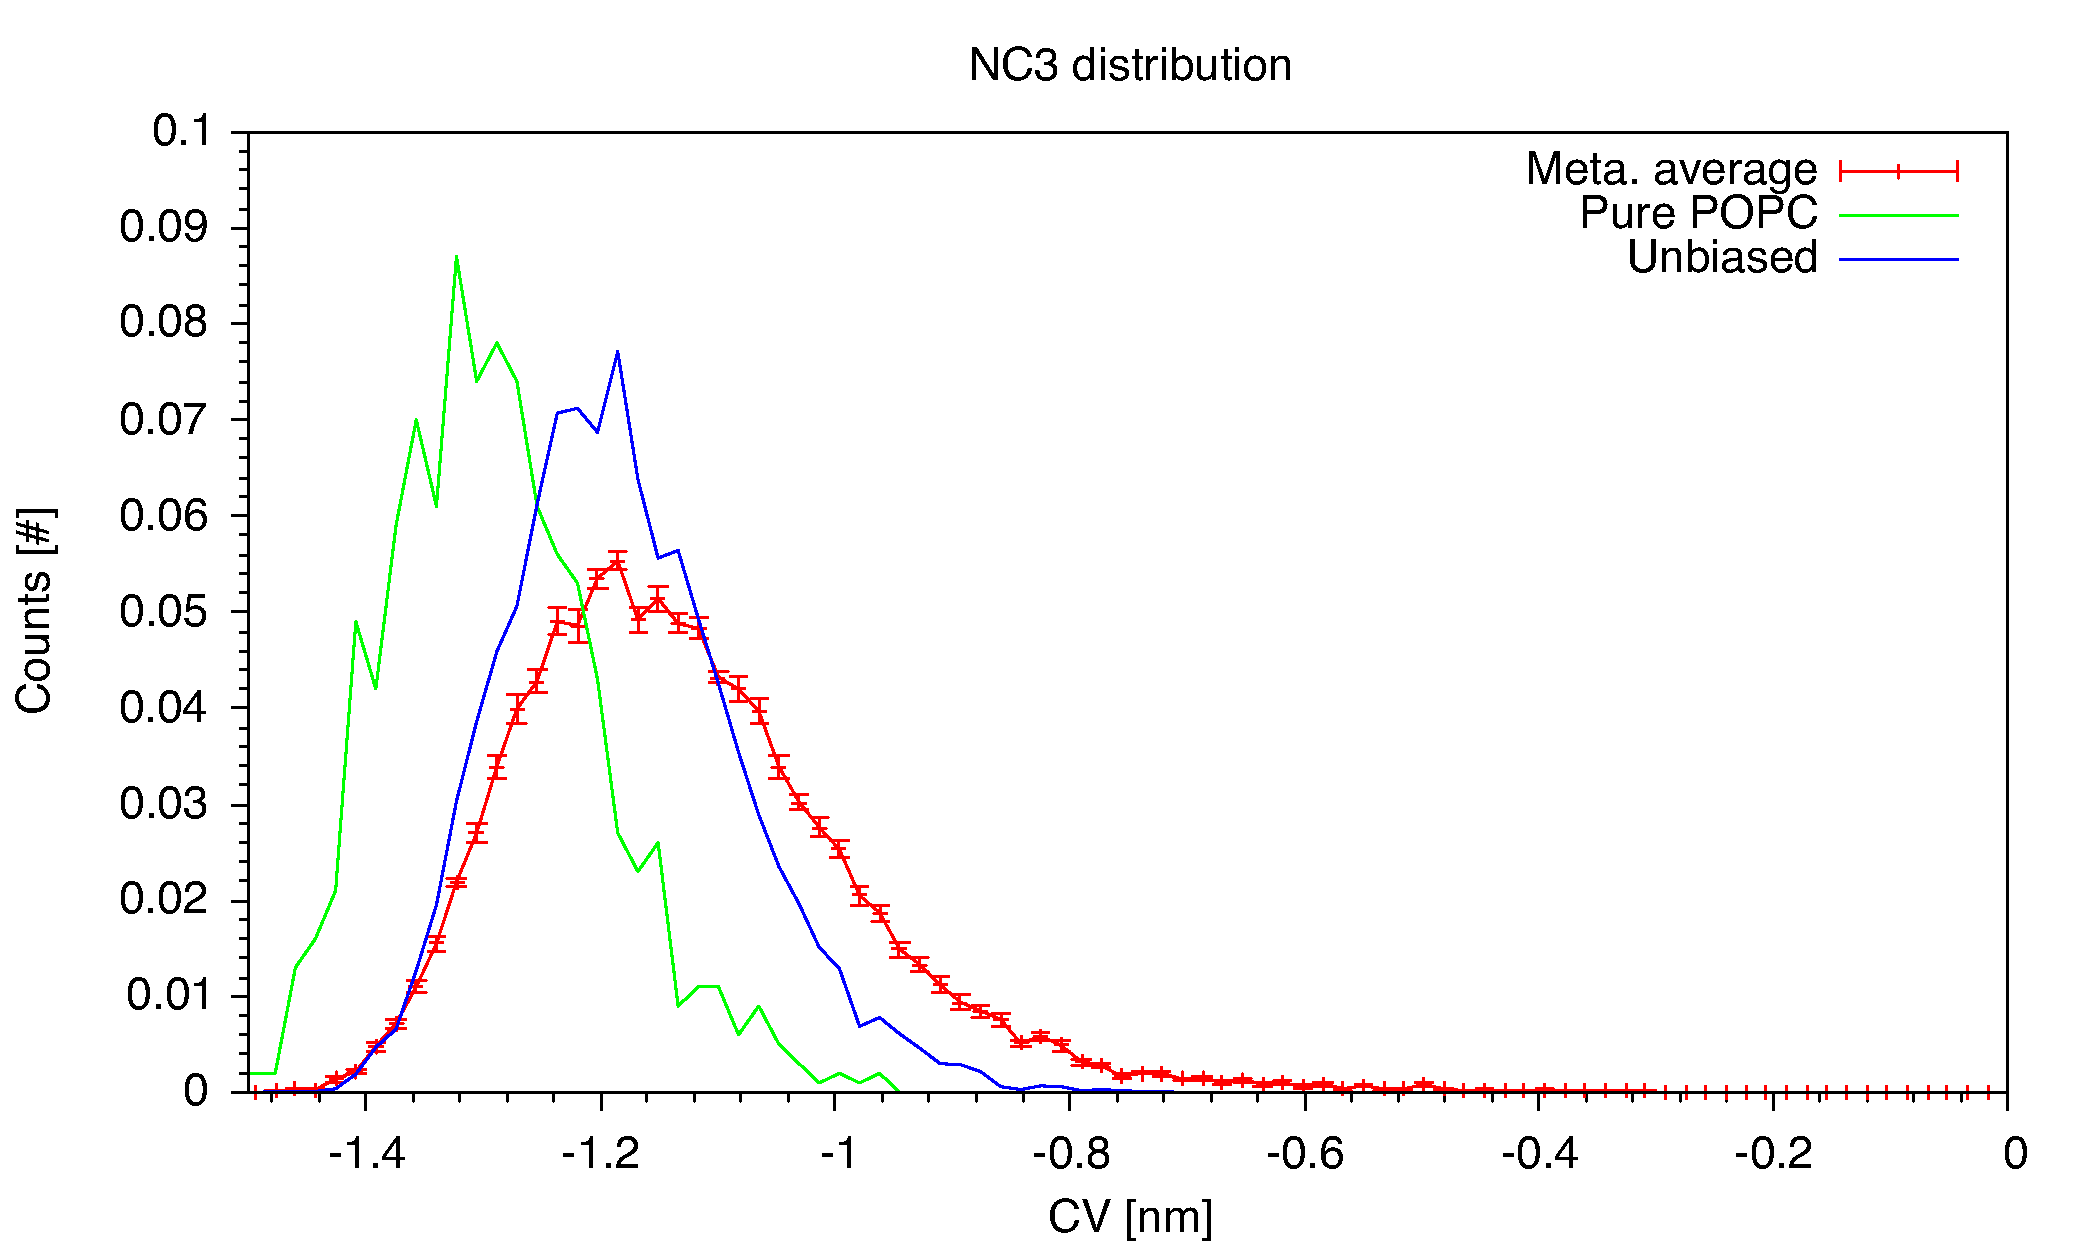
\includegraphics[width=\textwidth]{./img/results/minDistPatched}
	}\\%
	\subfloat[random NP]{
		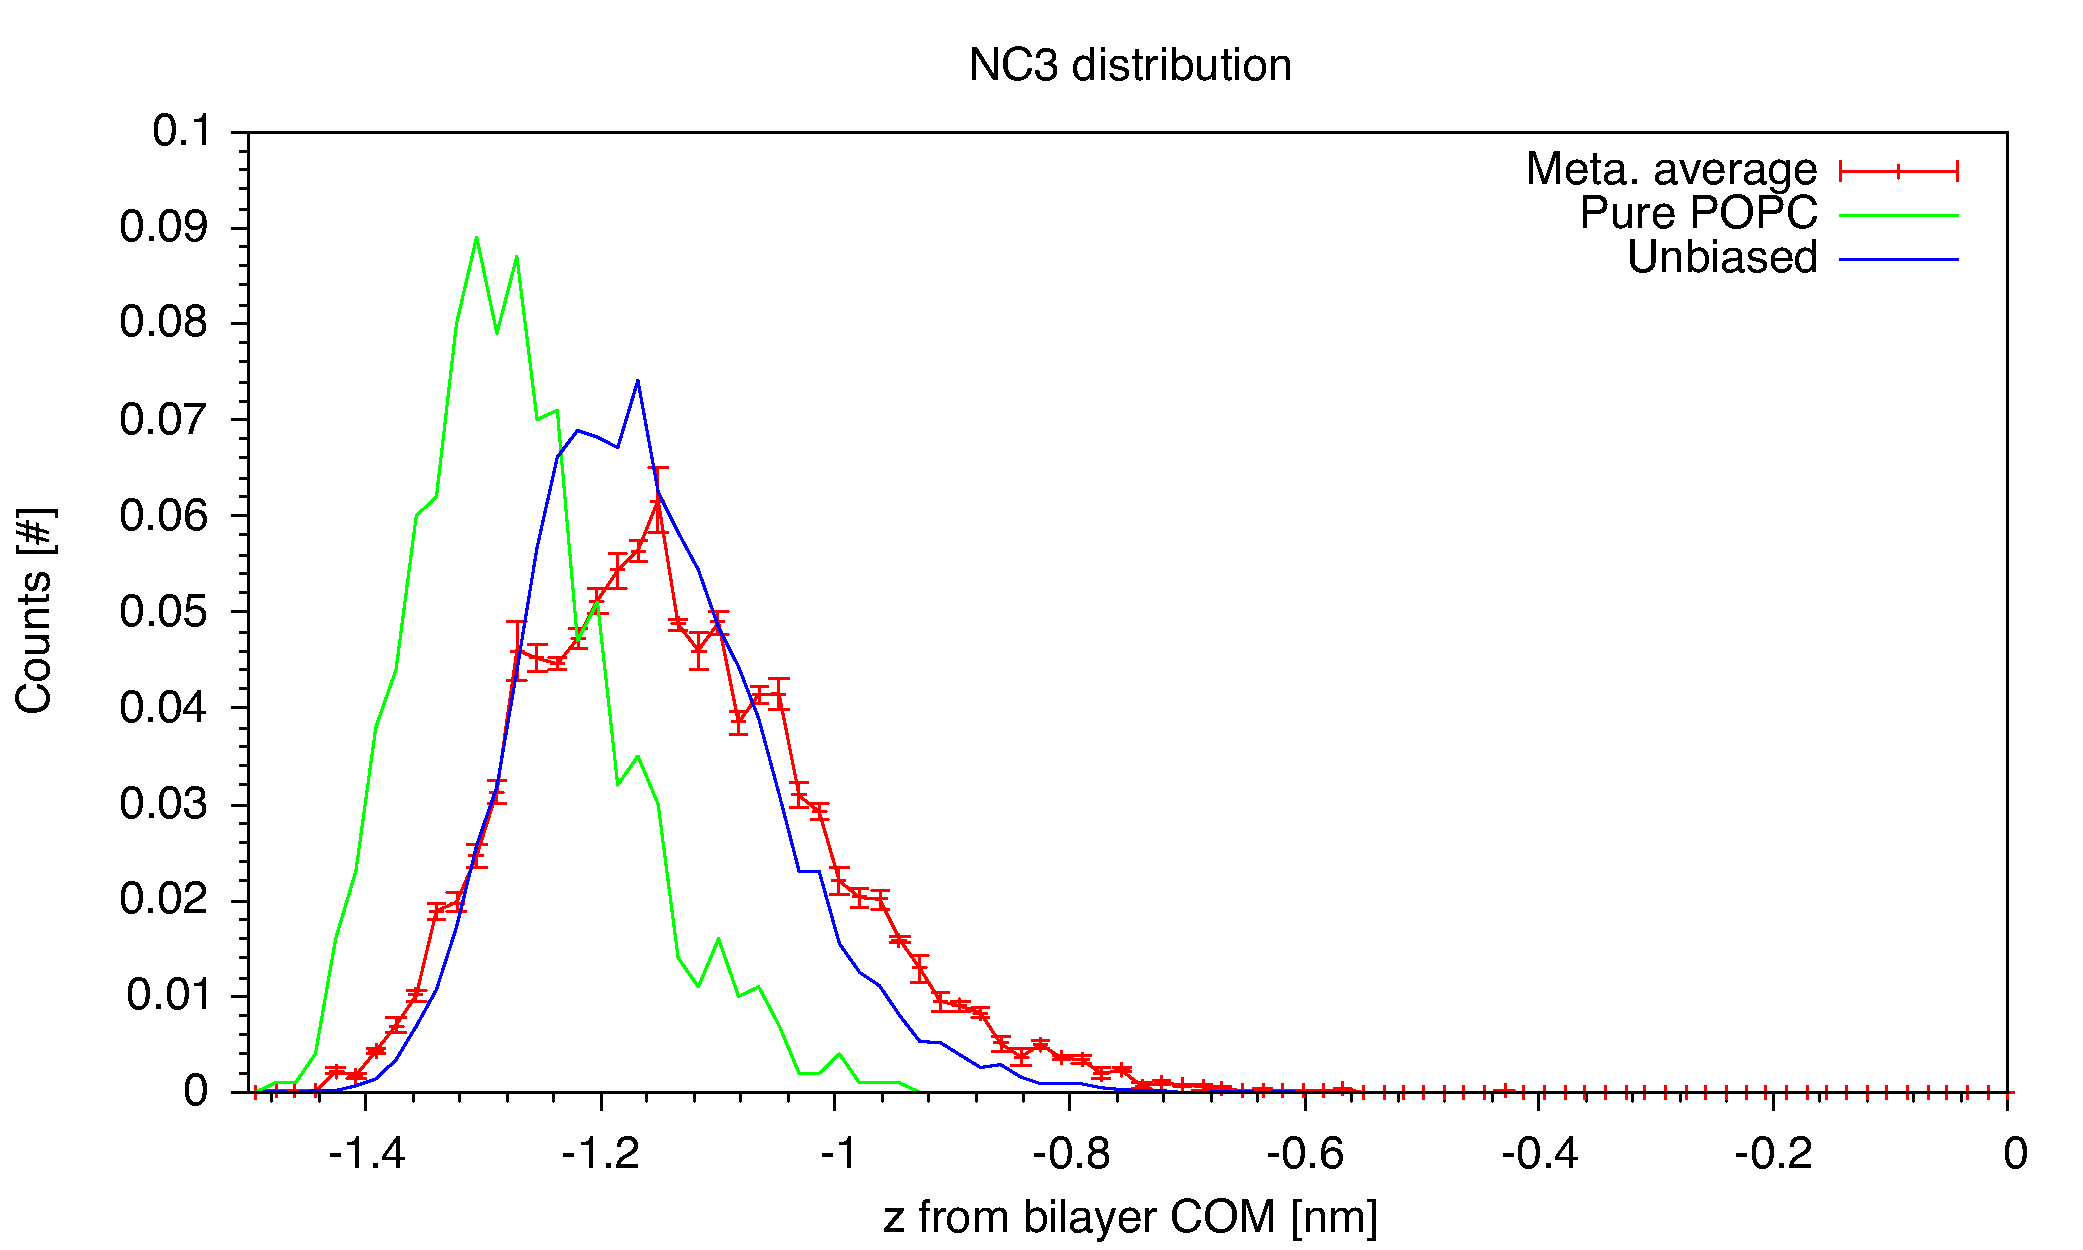
\includegraphics[width=\textwidth]{./img/results/minDistRandom11}
	}%
	\caption{Average distribution of the coline groups (NC3 beads) in the entrance leaflet closer to the bilayer \acs{COM} in function of the $z$ distance of the charged bead from the bilayer \acs{COM}; in comparison with an average over ten metadynamics runs, the unbiased run and a pure \acs{POPC} run for the striped \acs{NP} (a) and the random one (b).}
\end{figure}

%	NC3PatchedComparison	NC3RPComparison
\newgeometry{left=2.5cm,right=2.5cm}
\begin{figure}
	\center
	\subfloat[striped – model comparison]{
		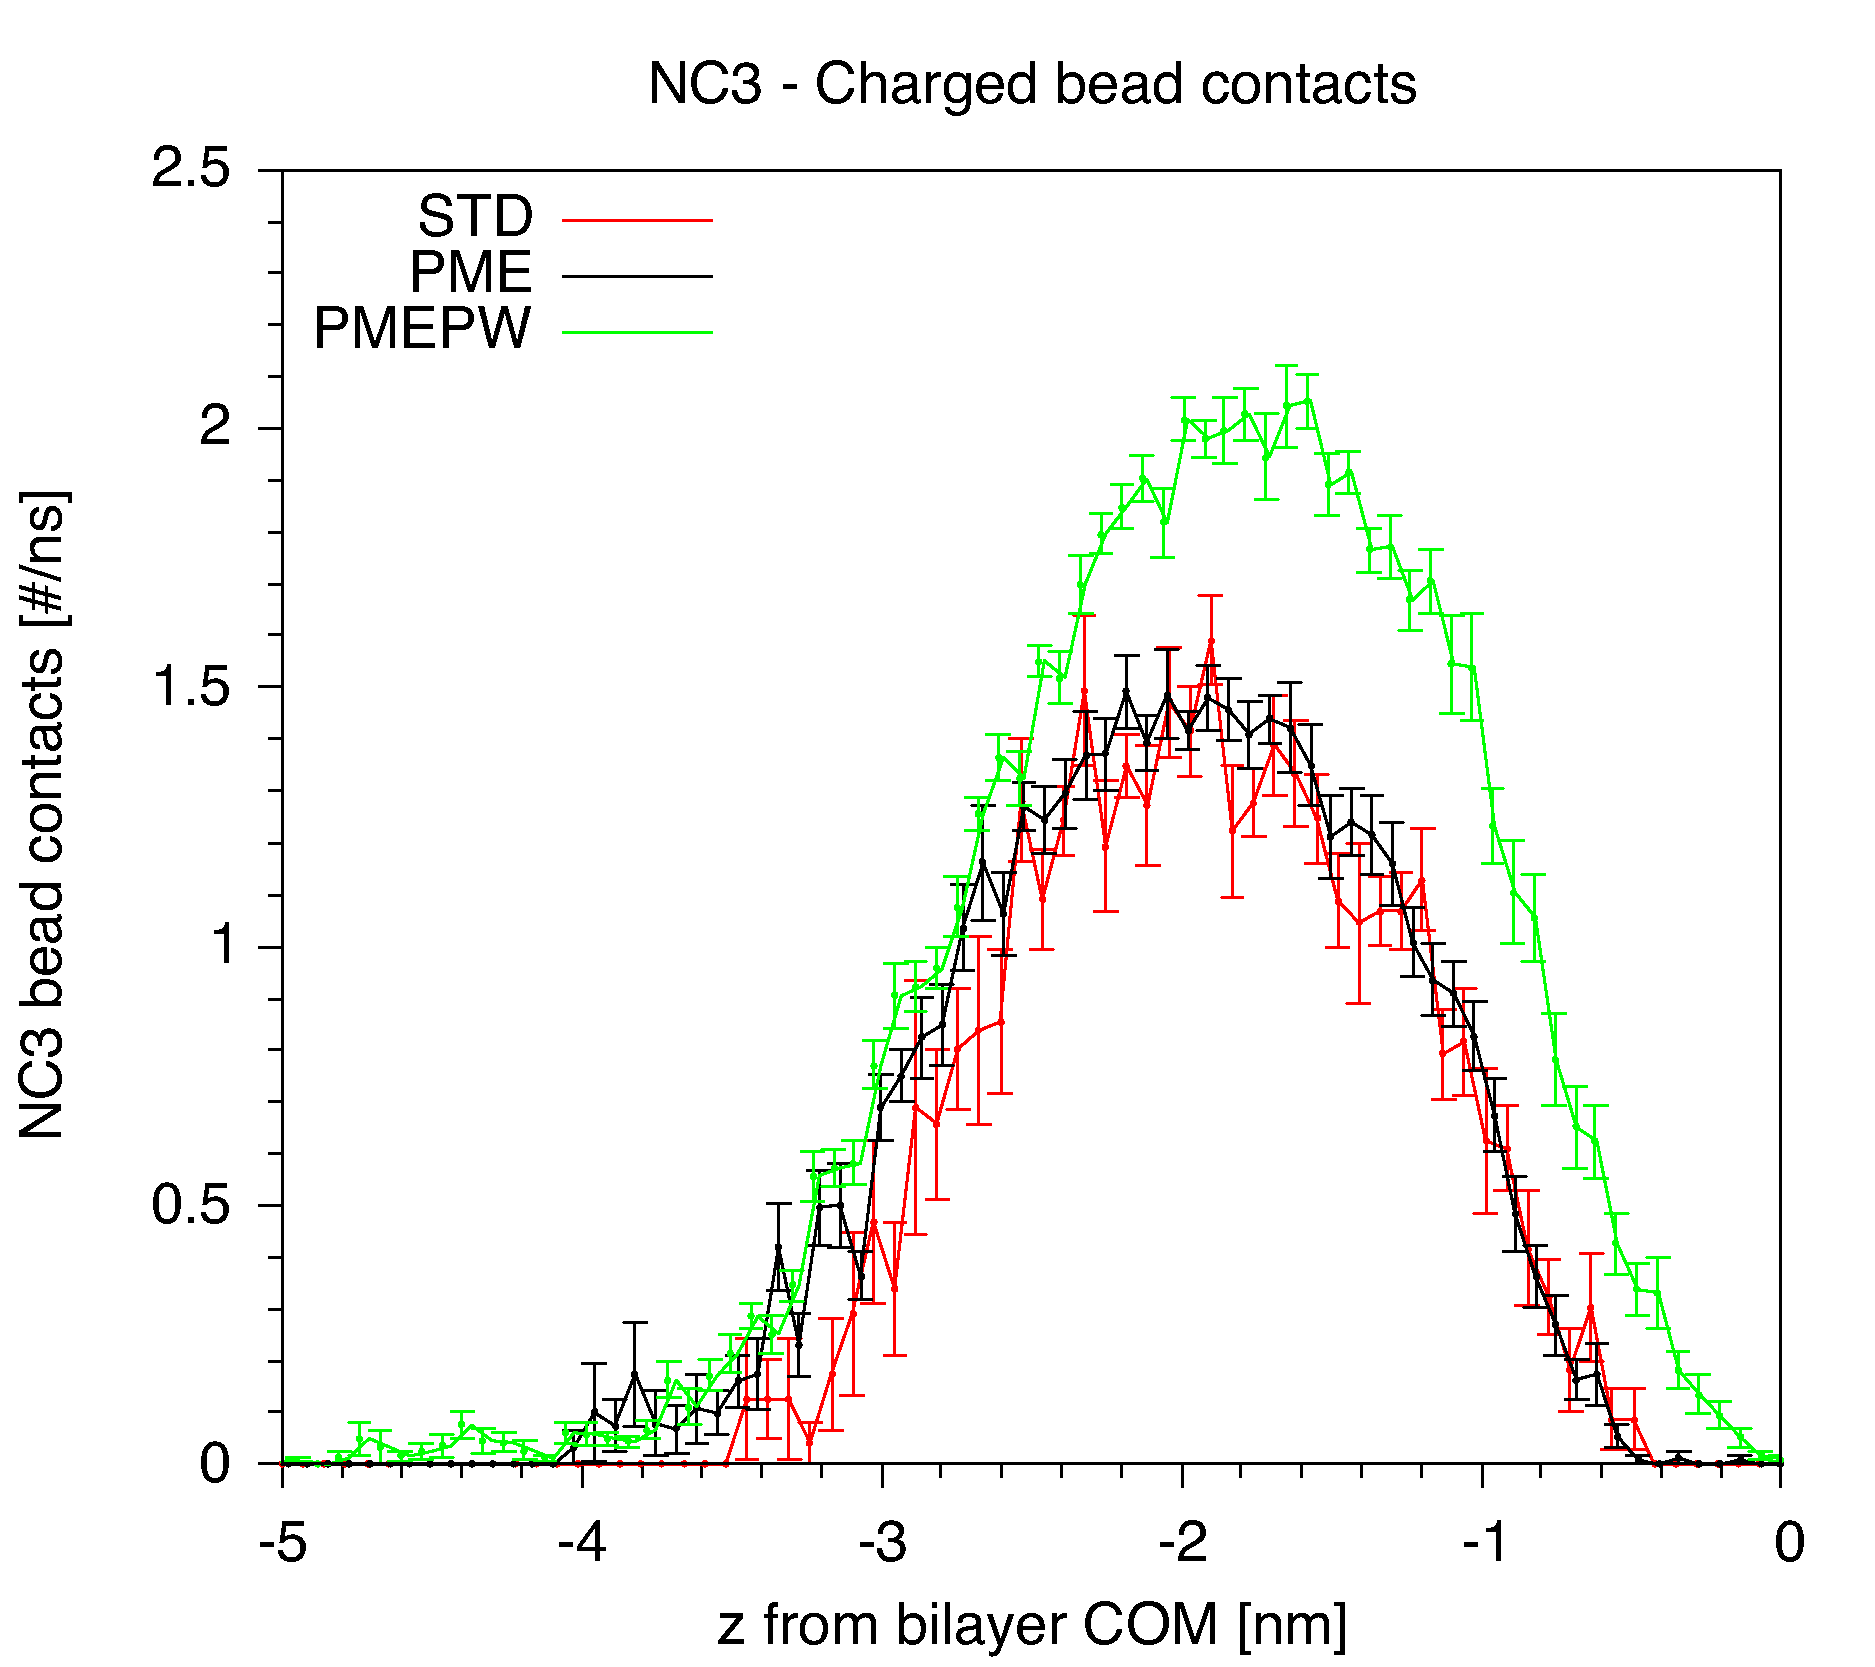
\includegraphics[width=0.5\textwidth]{./img/results/NC3PatchedComparison}
	}%
	\subfloat[striped – random comparison]{
		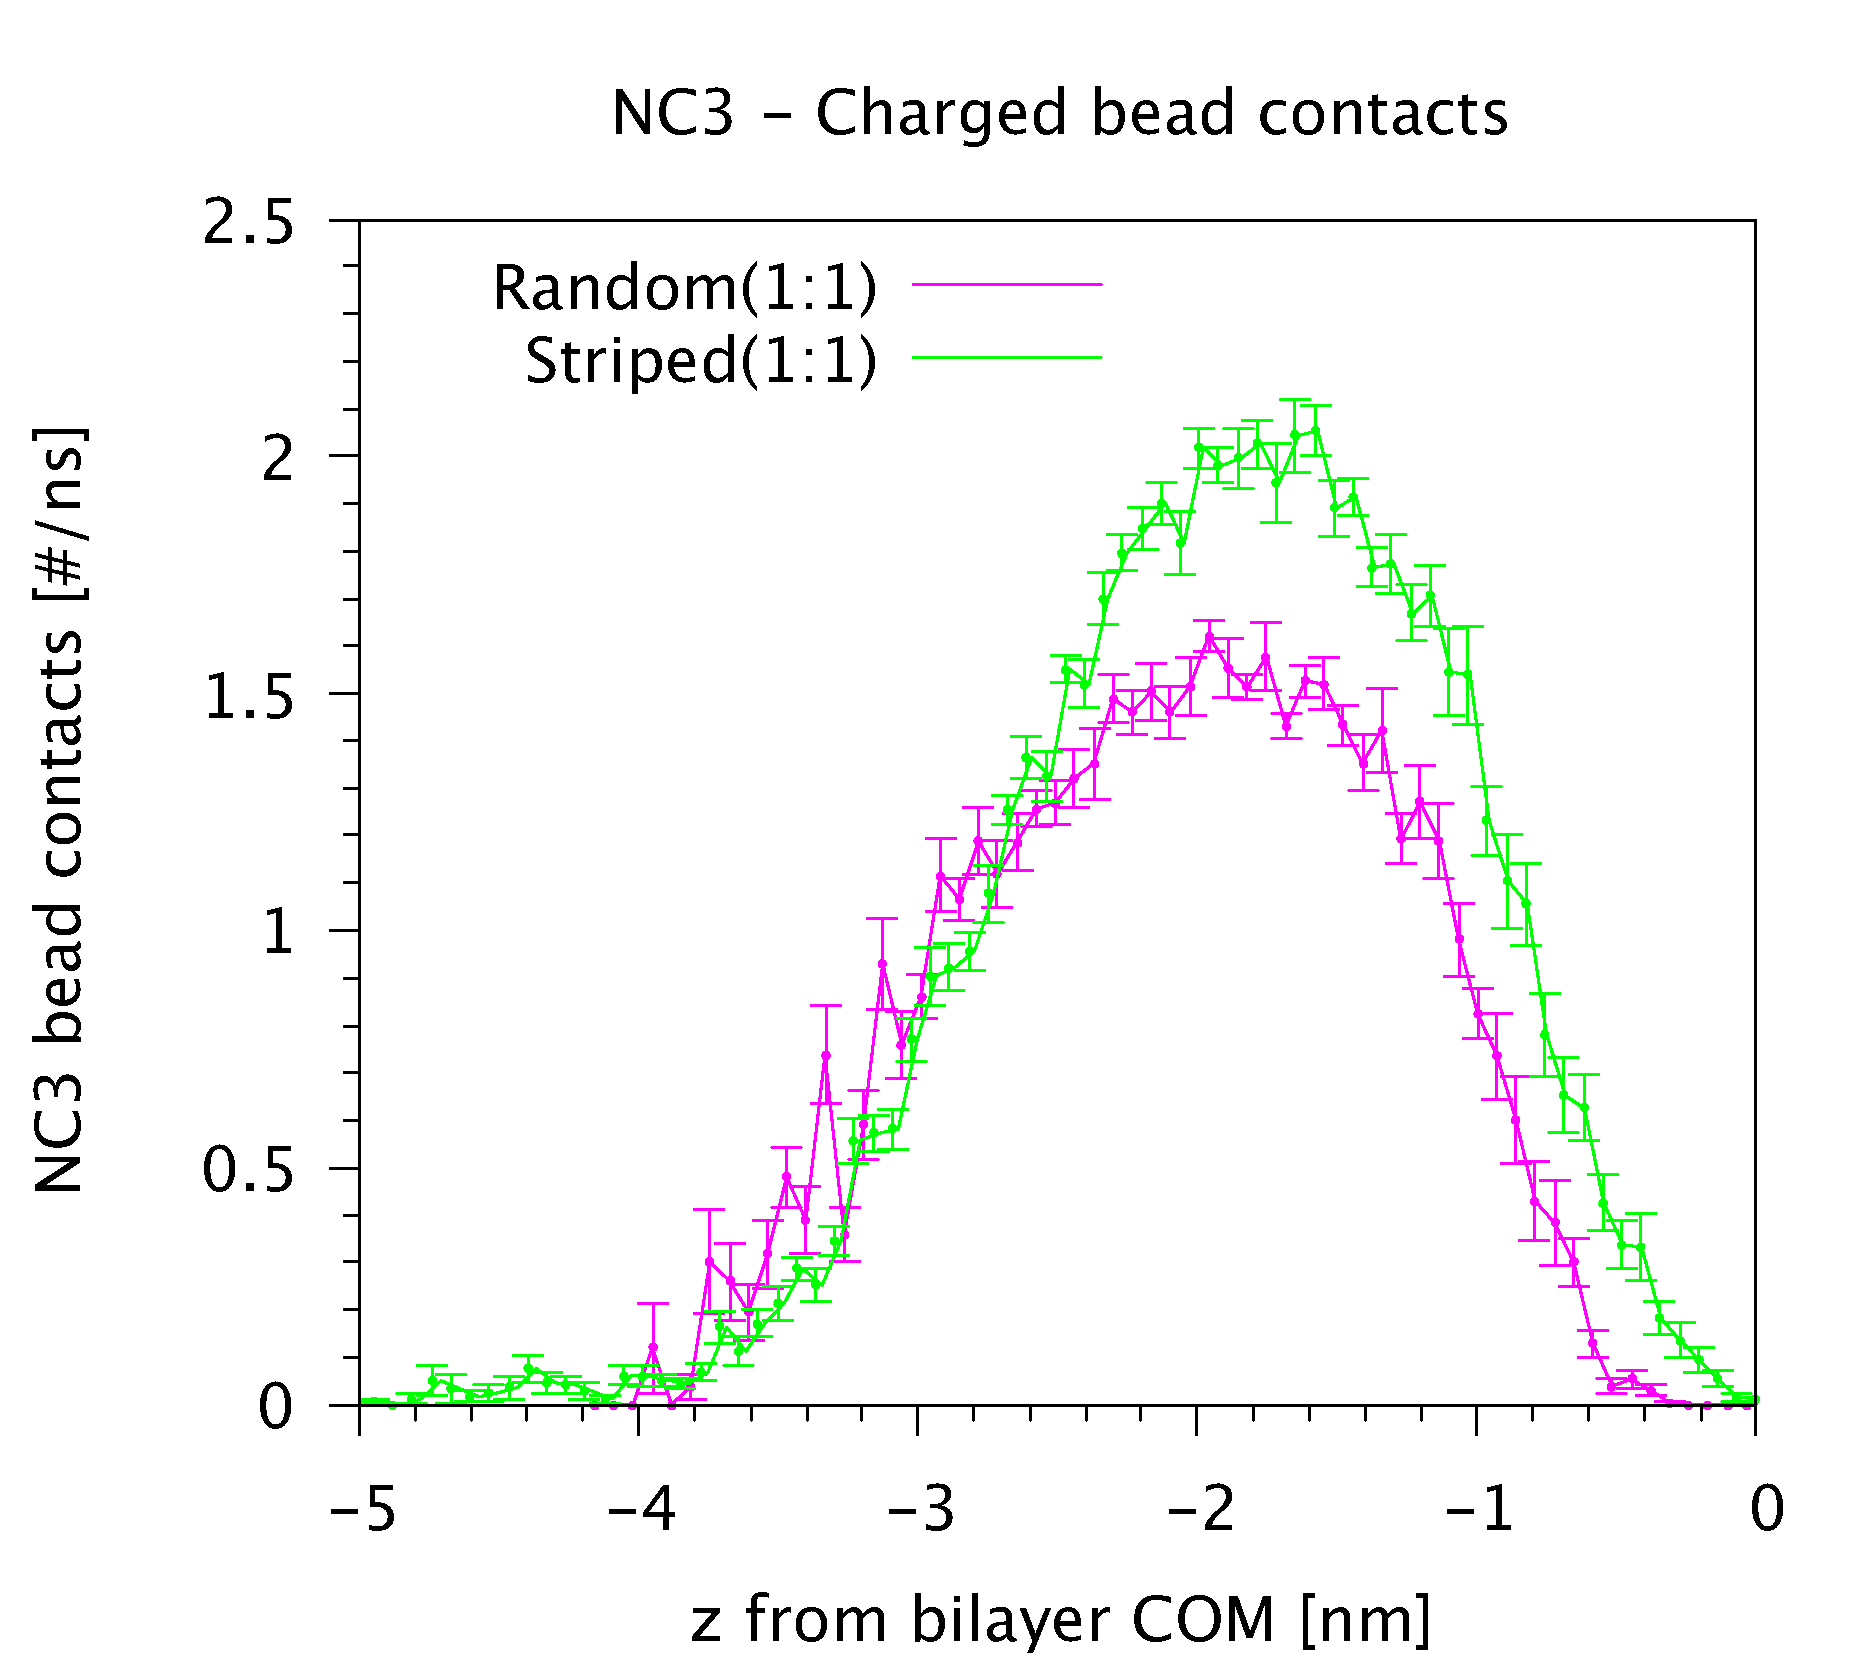
\includegraphics[width=0.5\textwidth]{./img/results/NC3RPComparison}
	}%
	\caption{Number of contacts per ns between coline group (NC3 bead) and the charged bead in function of the $z$ distance of the charged bead from the bilayer \acs{COM}. (a) For the striped \acs{NP} in comparison with different models. (b) In comparison between the striped and the random \acs{NP}s.}
\end{figure}
\restoregeometry

\section{Effects of metadynamics}
%Quanto la metadinamica sia distrittiva: comparazione tra rum unbiased e biased

% 	minDistHydroPatched		minDistHydroRandom11
\begin{figure}[p]
	\center
	\subfloat[striped NP]{
		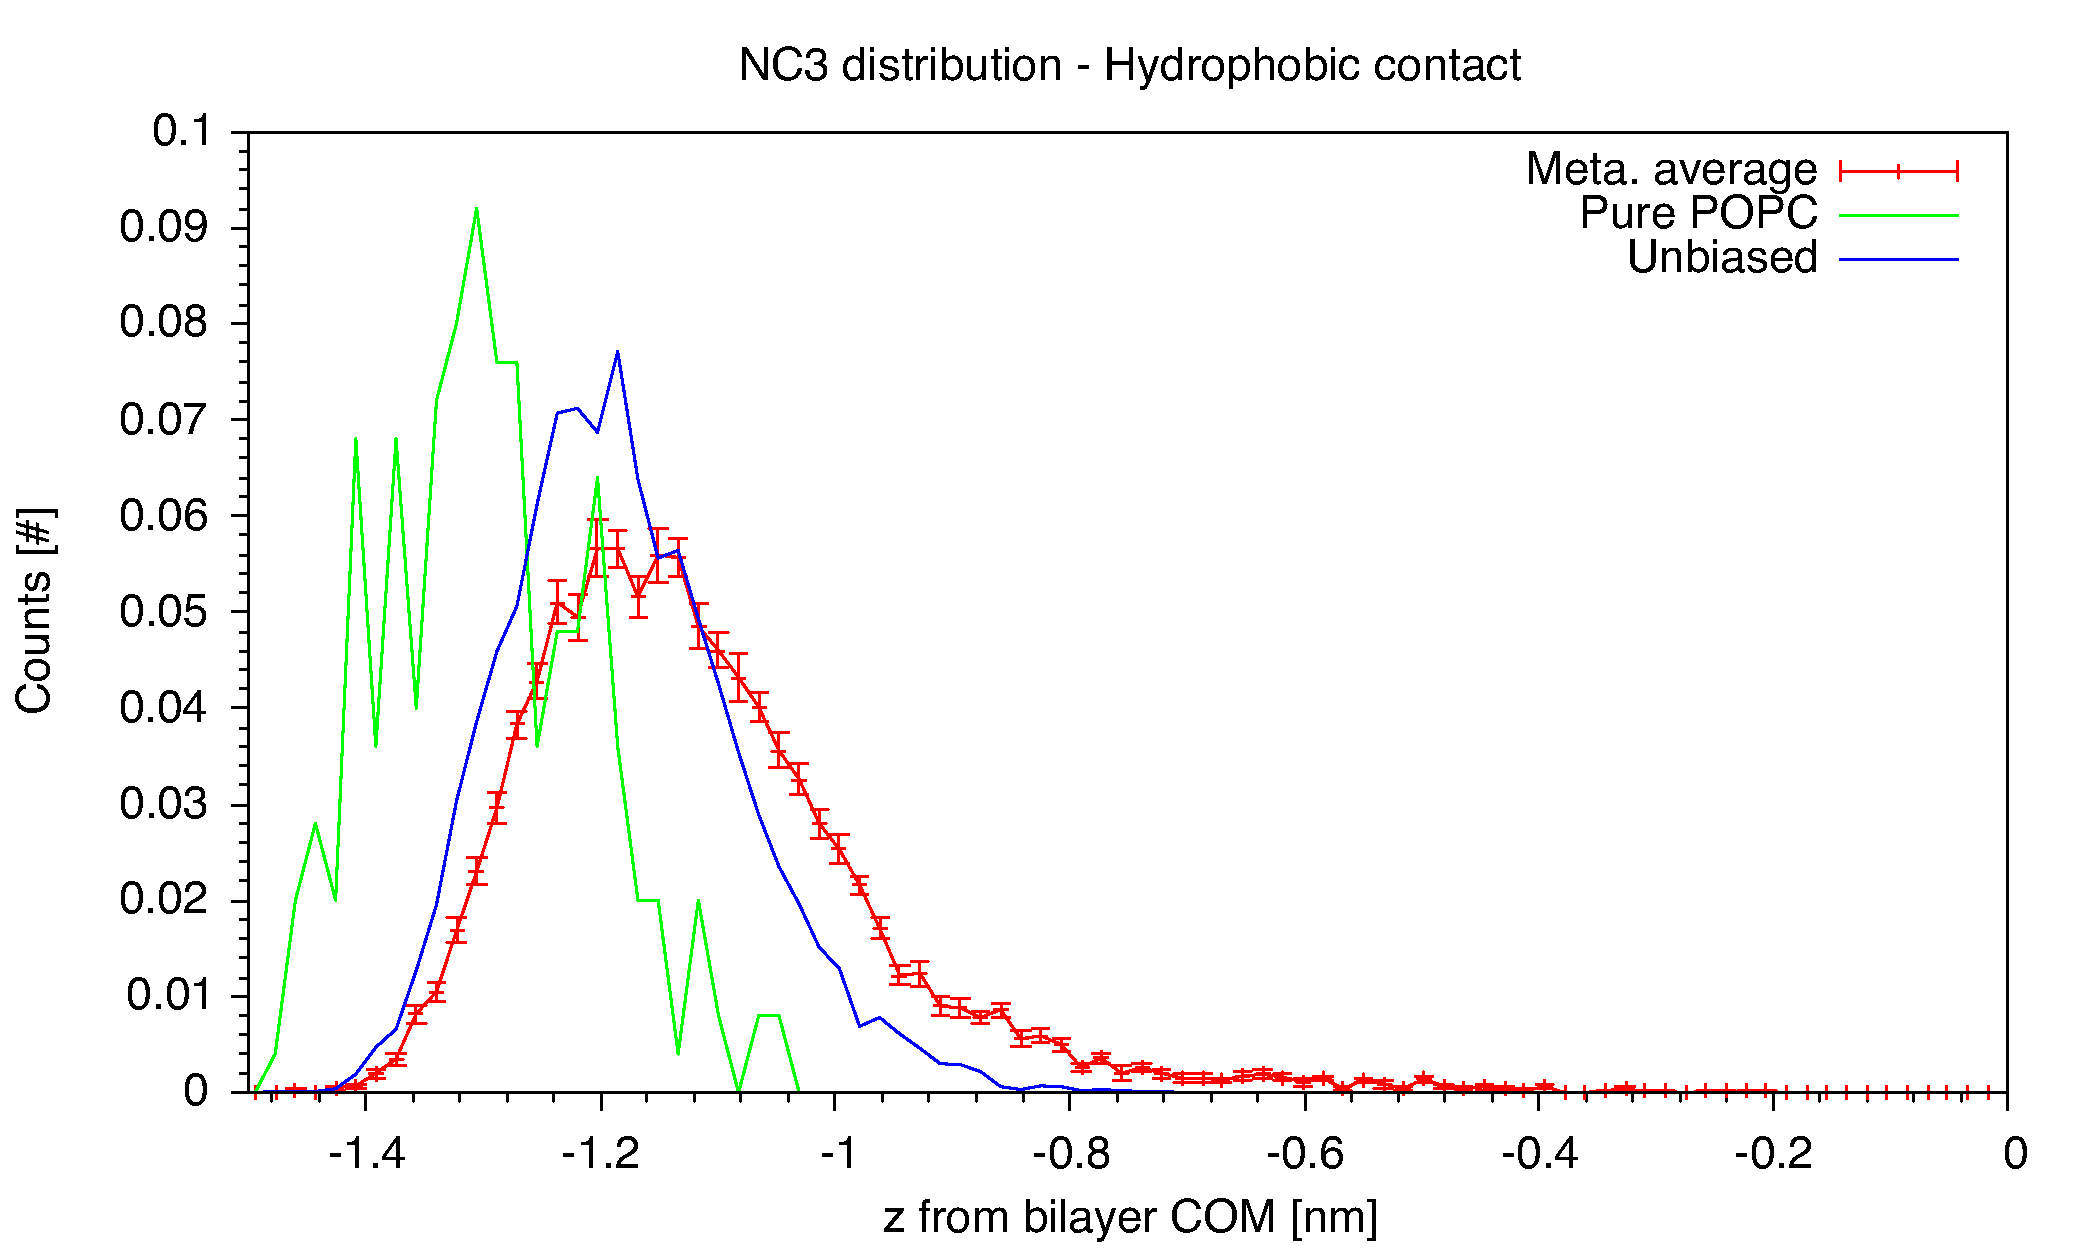
\includegraphics[width=\textwidth]{./img/results/minDistHydroPatched}
	}\\%
	\subfloat[random NP]{
		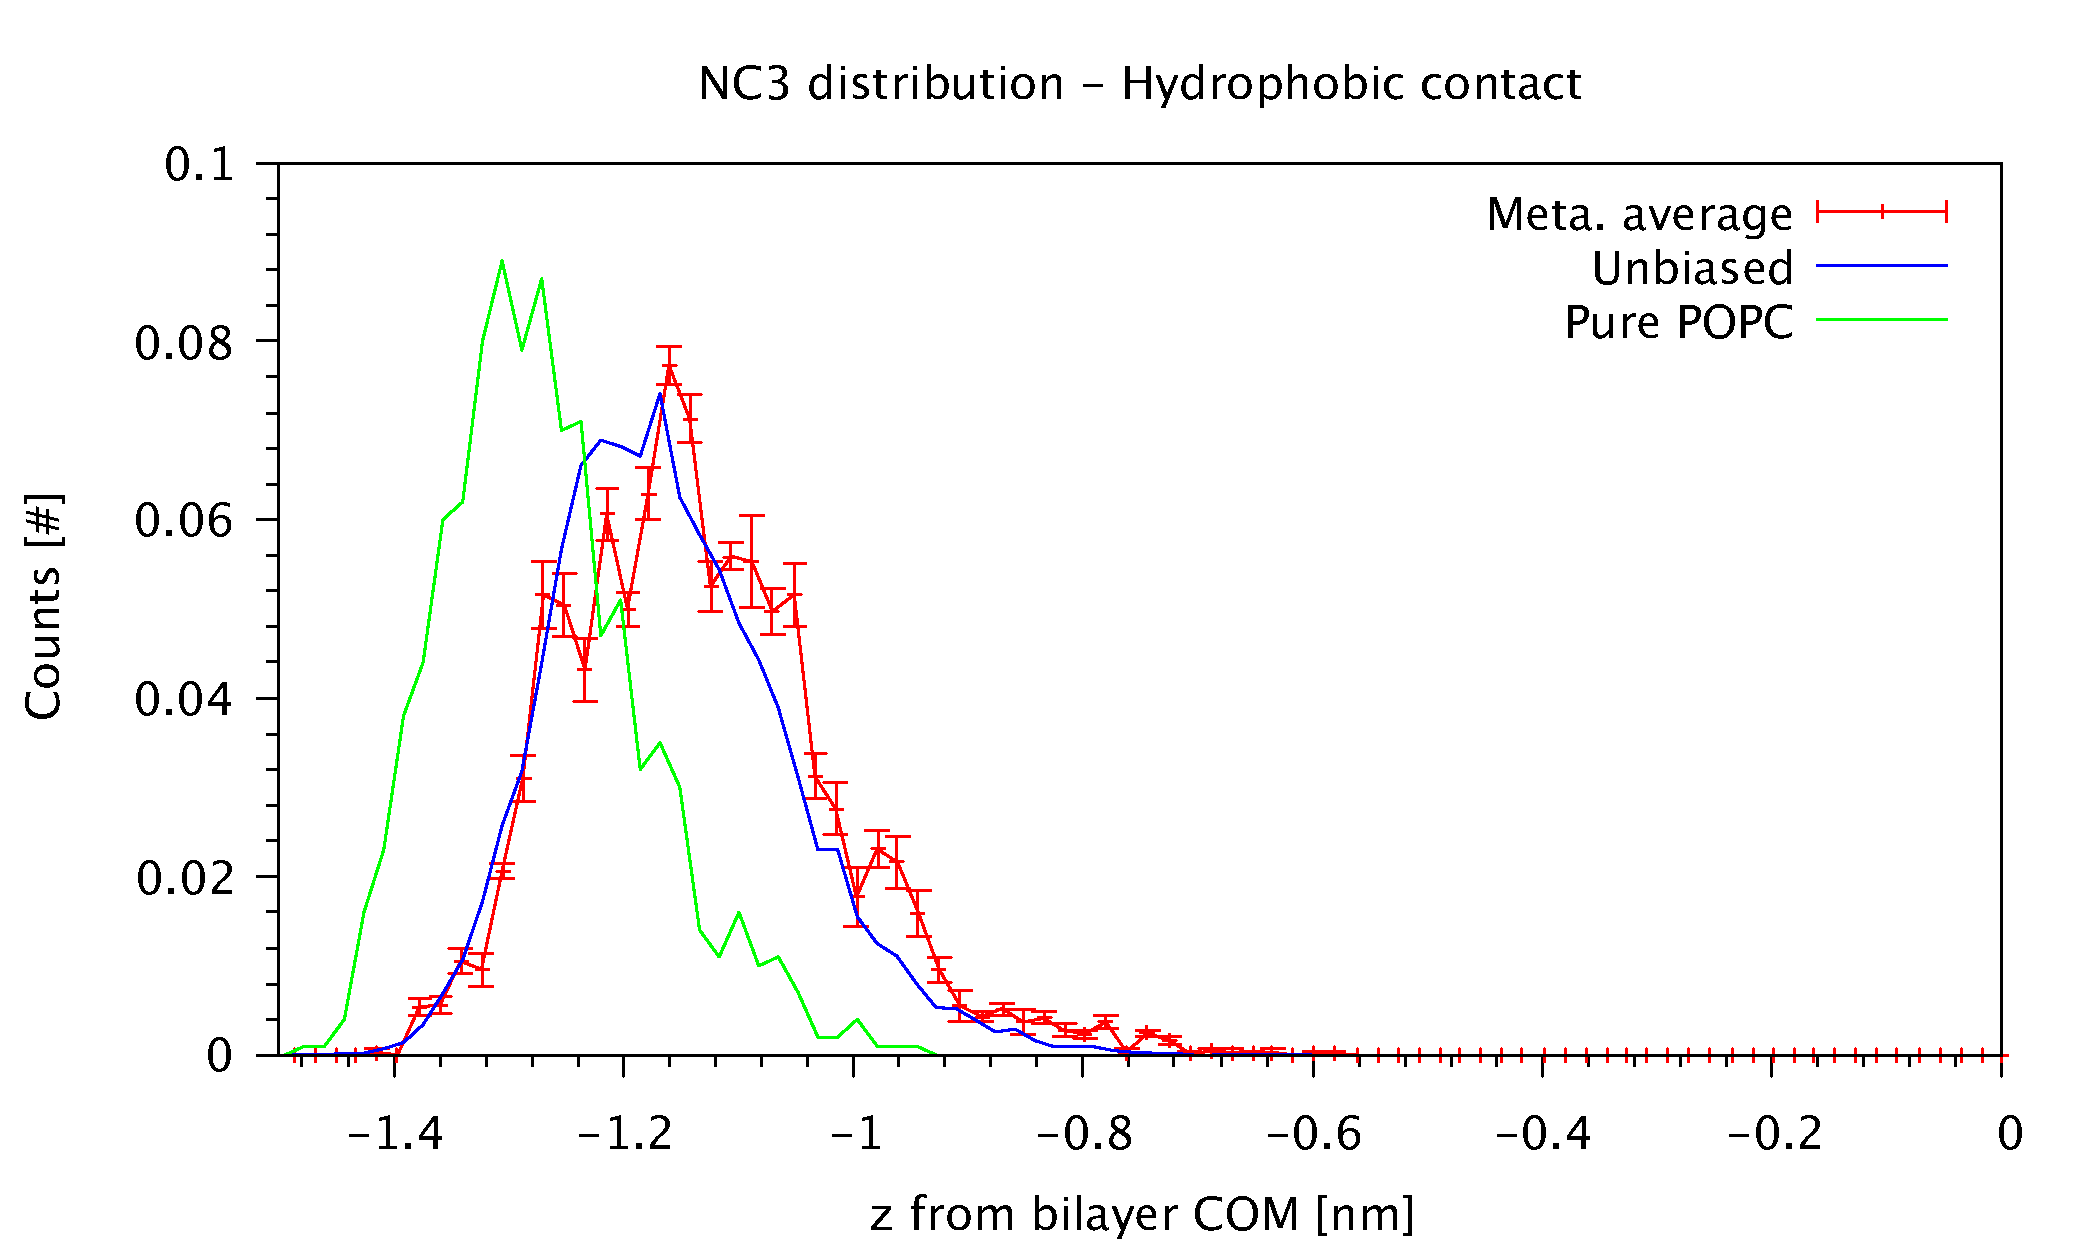
\includegraphics[width=\textwidth]{./img/results/minDistHydroRandom11}
	}%
	\caption{Average distribution of the coline groups (NC3 beads) in the entrance leaflet closer to the bilayer \acs{COM} in function of the $z$ distance of the charged bead from the bilayer \acs{COM}; in comparison with an average over ten metadynamics runs in the hydrophobic contact only, the unbiased run and a pure \acs{POPC} run for the striped \acs{NP} (a) and the random one (b).}
\end{figure}

%	patchedPWContact	randon11PWContact
% 	patchedNC3Contact
\newgeometry{left=2.5cm,right=2.5cm}
\begin{figure}[p]
	\center
	\subfloat[striped NP]{
		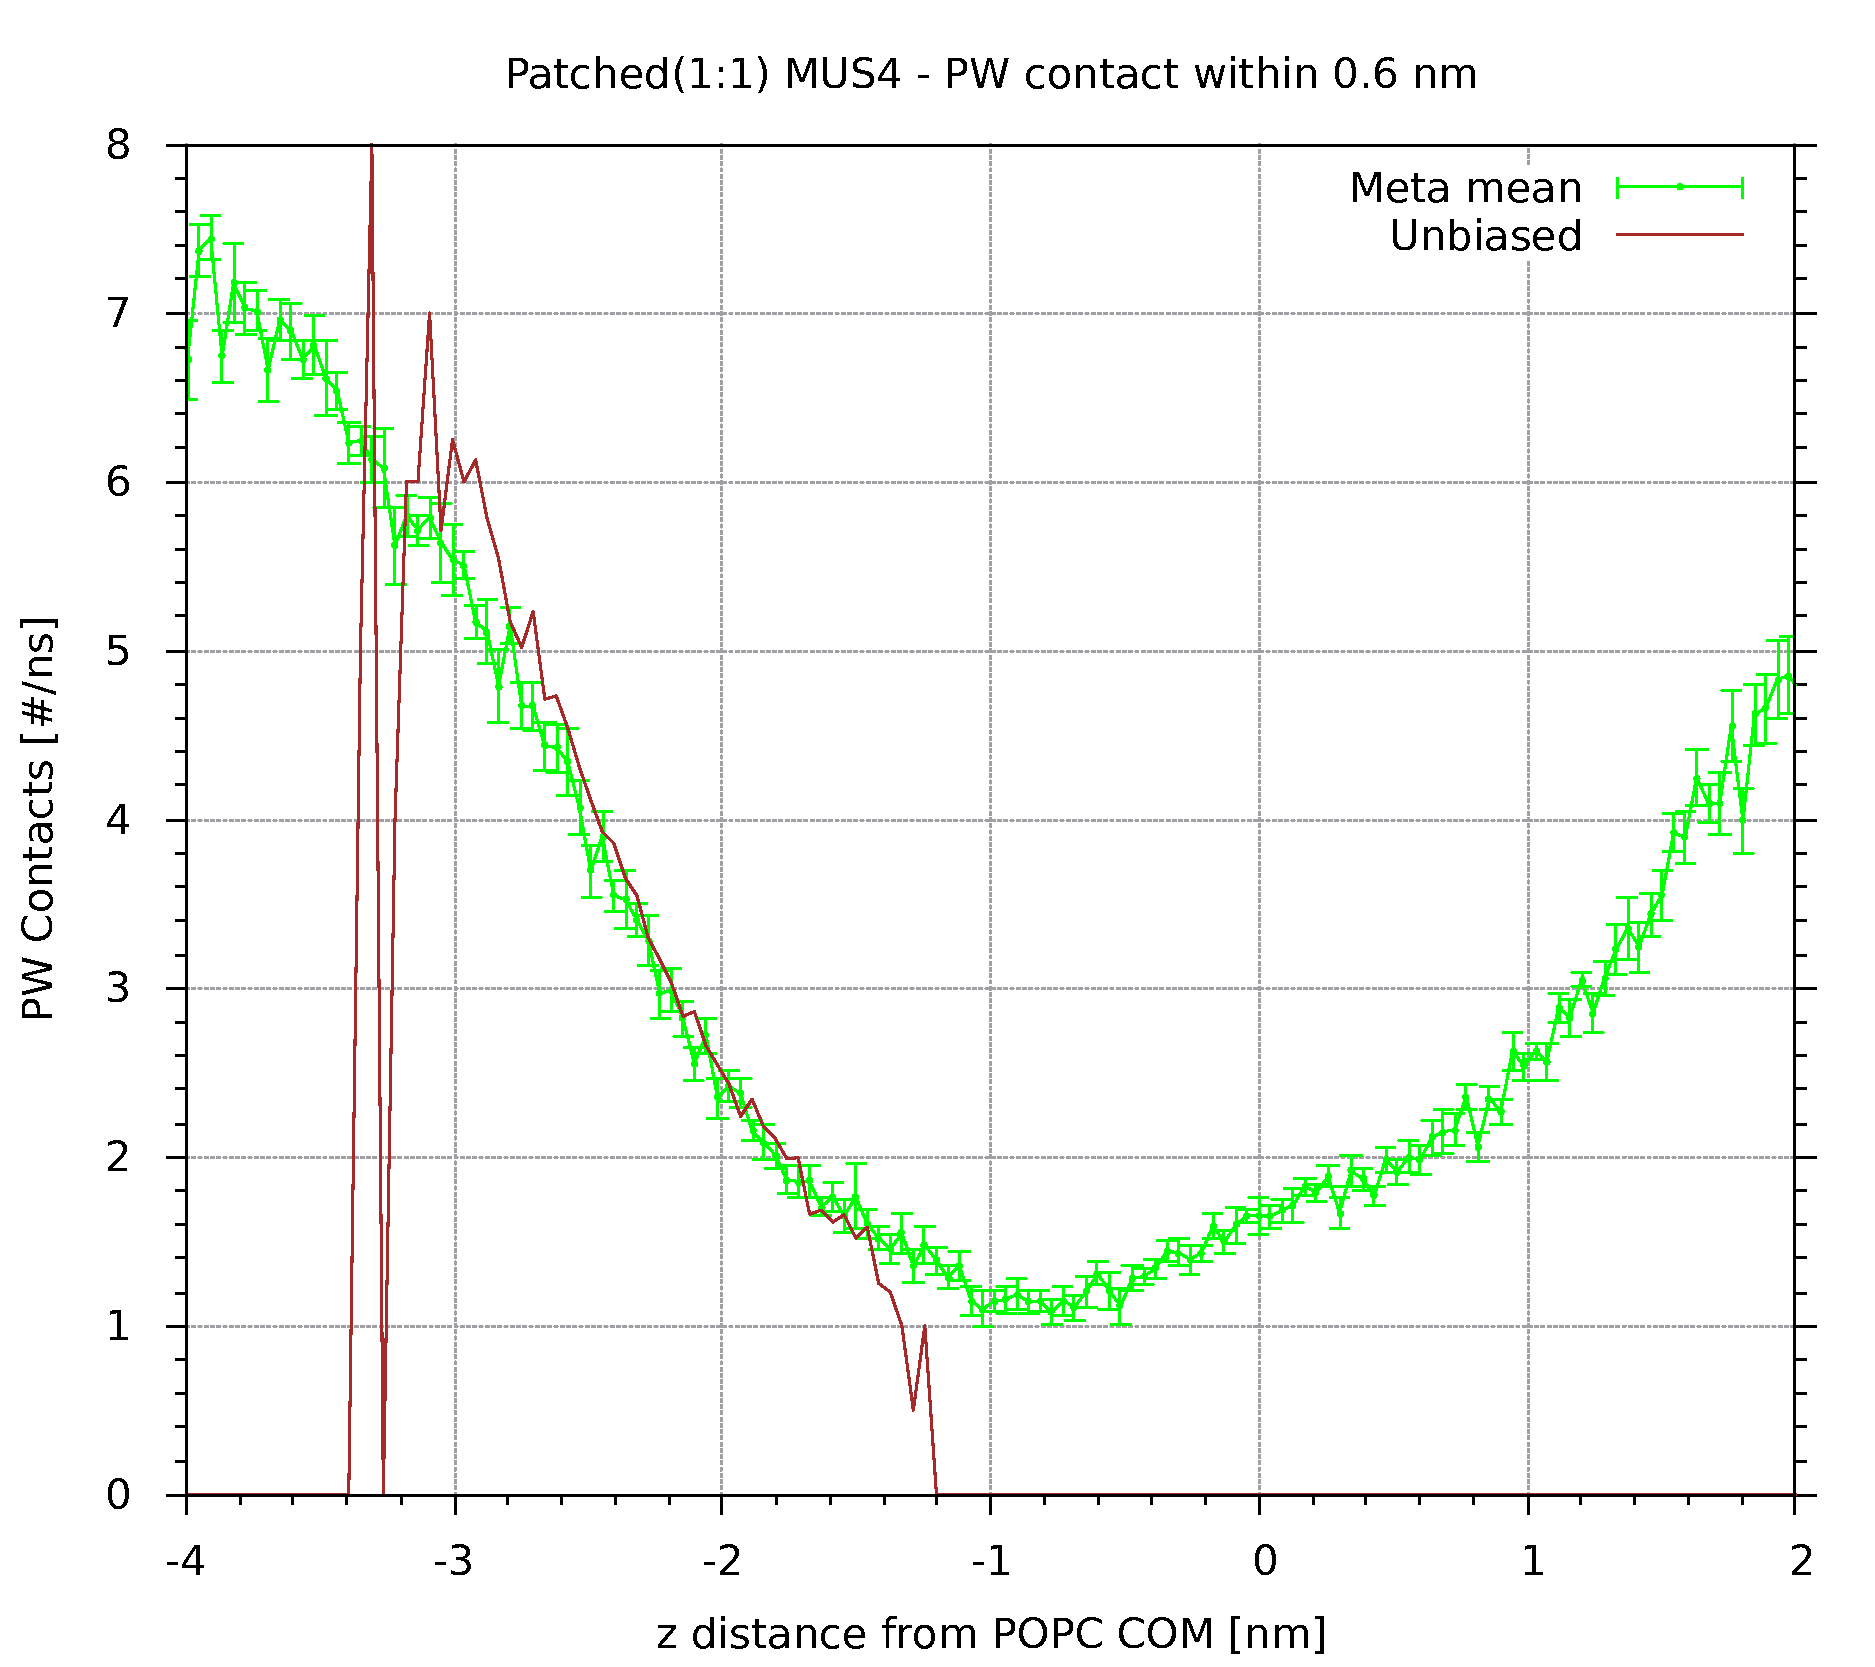
\includegraphics[width=0.5\textwidth]{./img/results/patchedPWContact}
	}%
	\subfloat[random NP]{
		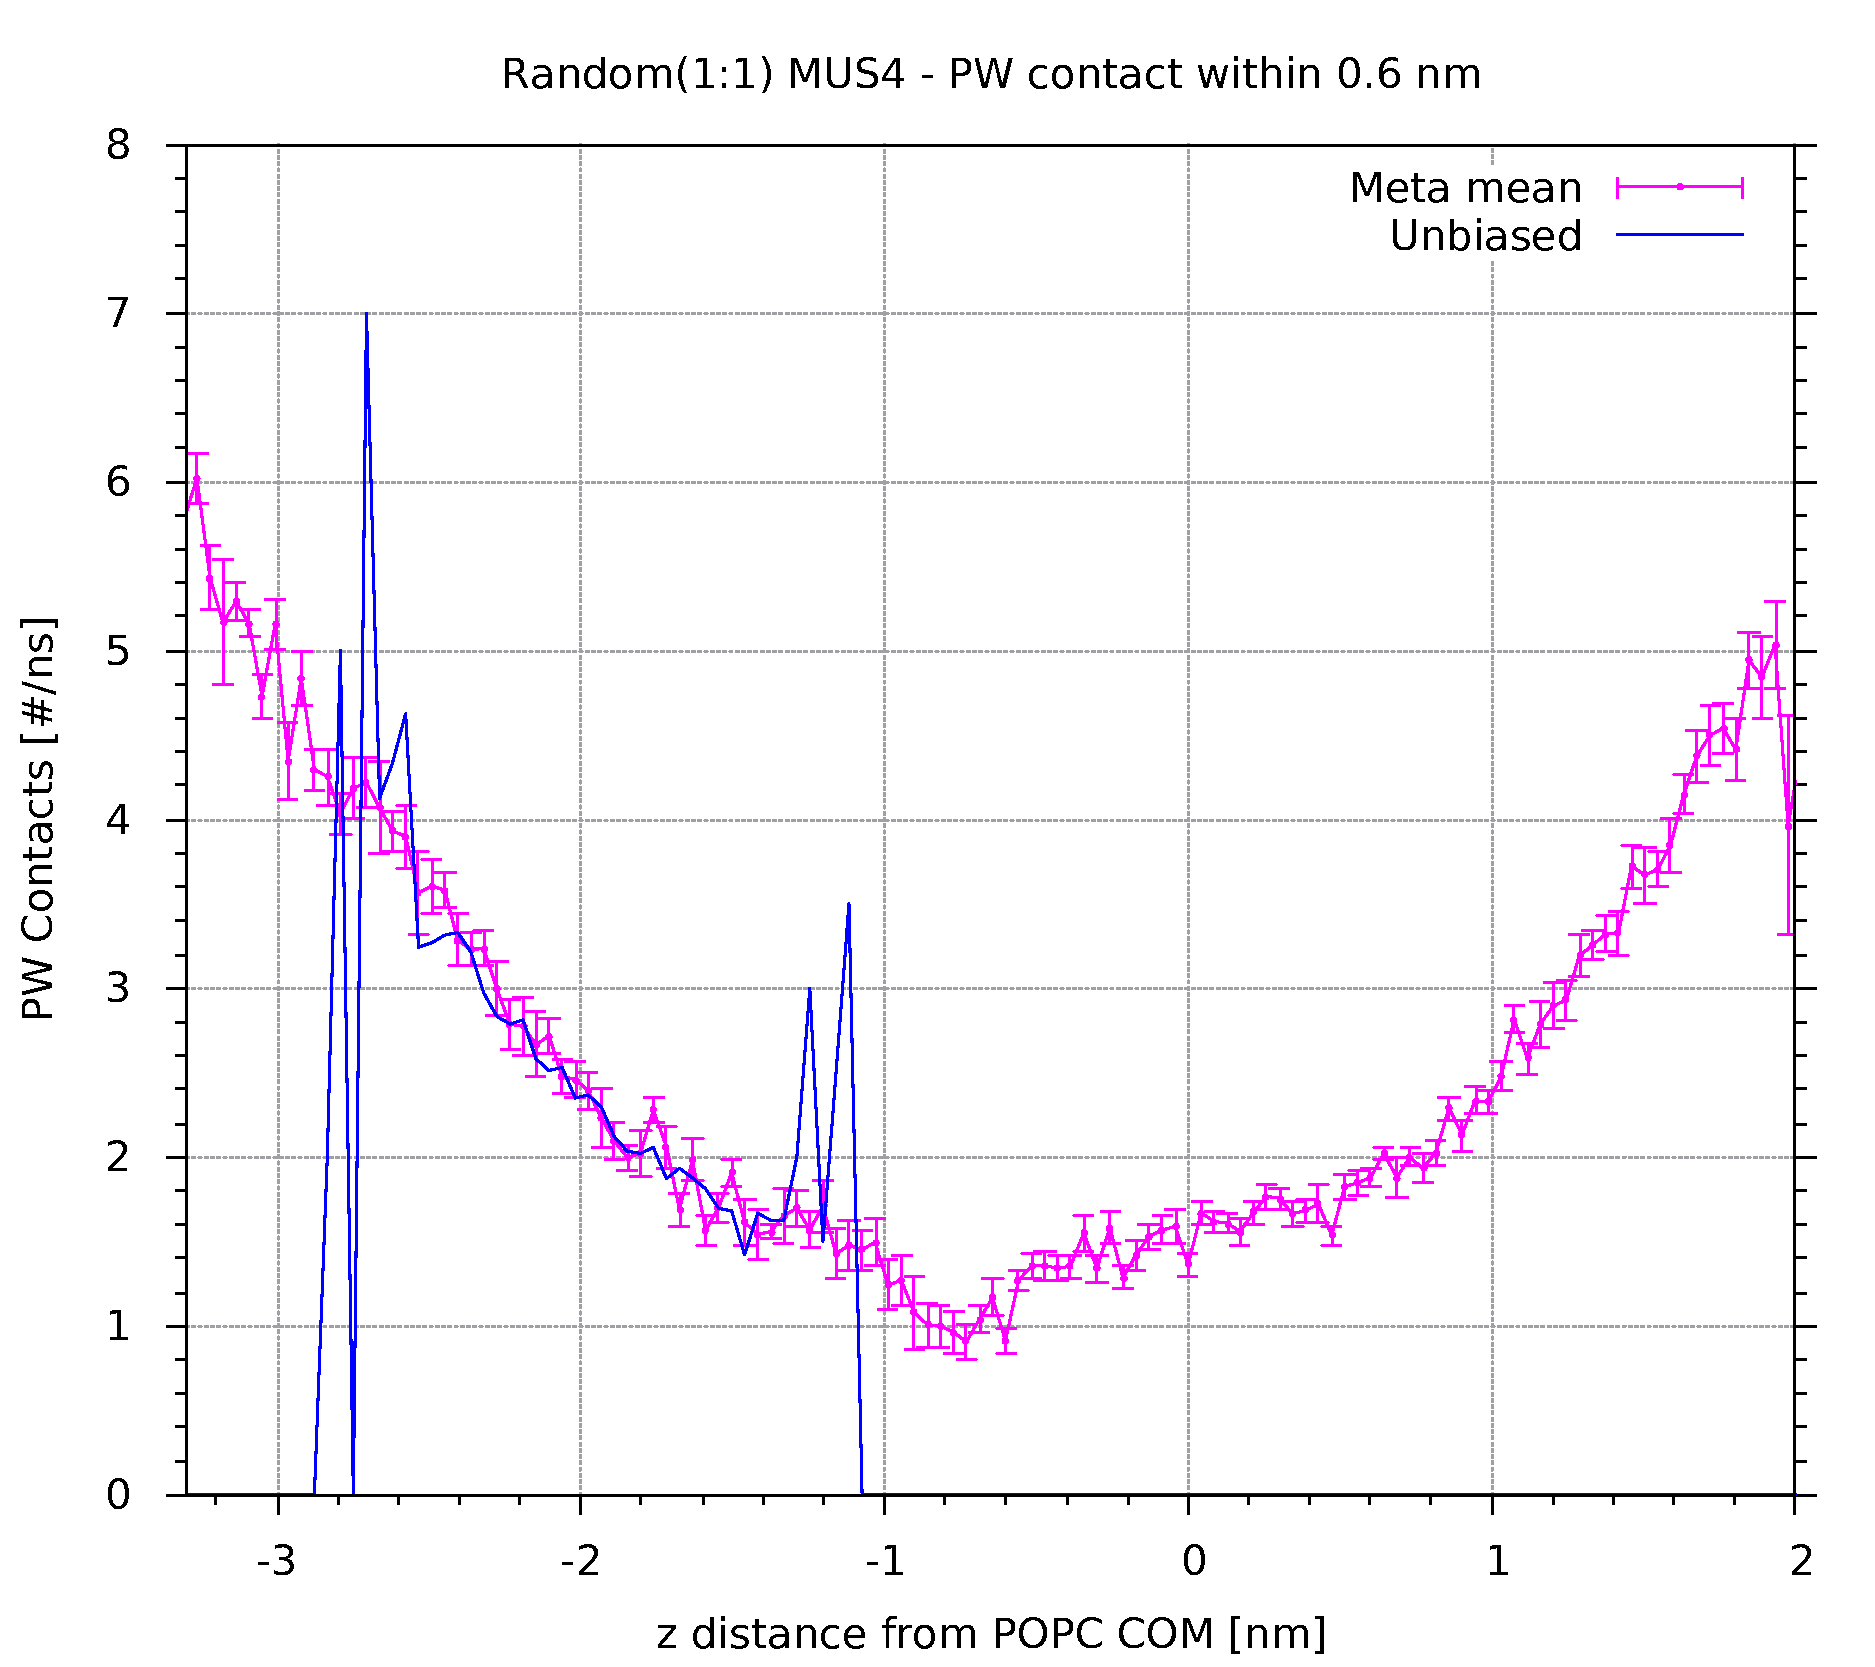
\includegraphics[width=0.5\textwidth]{./img/results/randon11PWContact}
	}\\%
	\subfloat[striped NP]{
		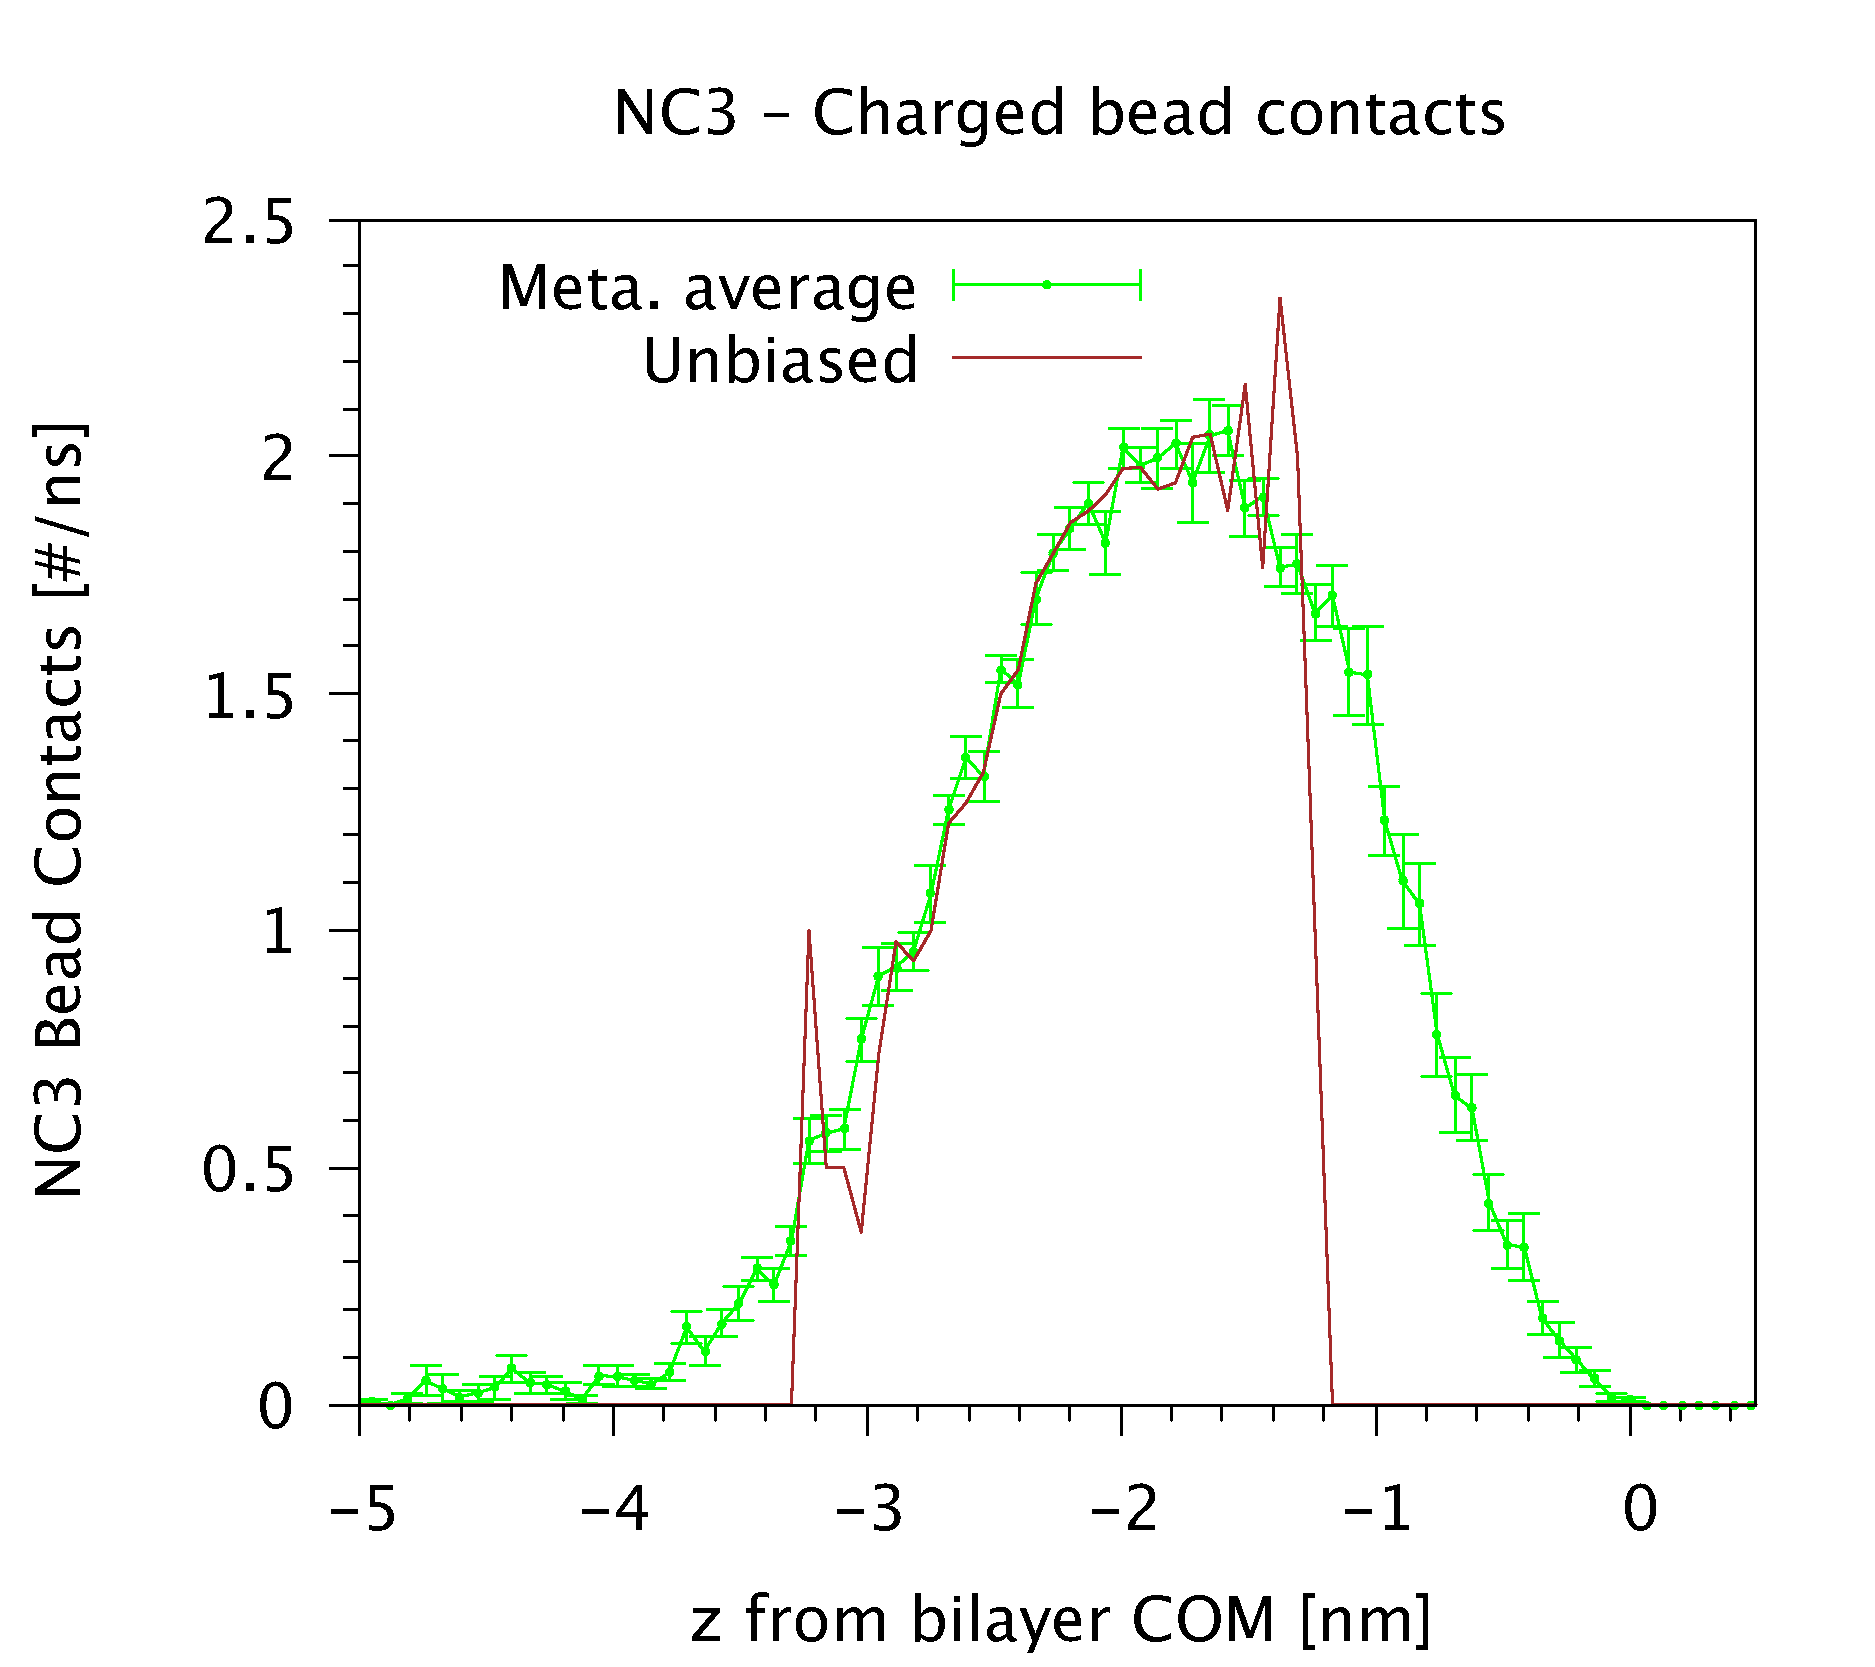
\includegraphics[width=0.5\textwidth]{./img/results/patchedNC3Contact}
	}%
	\subfloat[random NP]{
		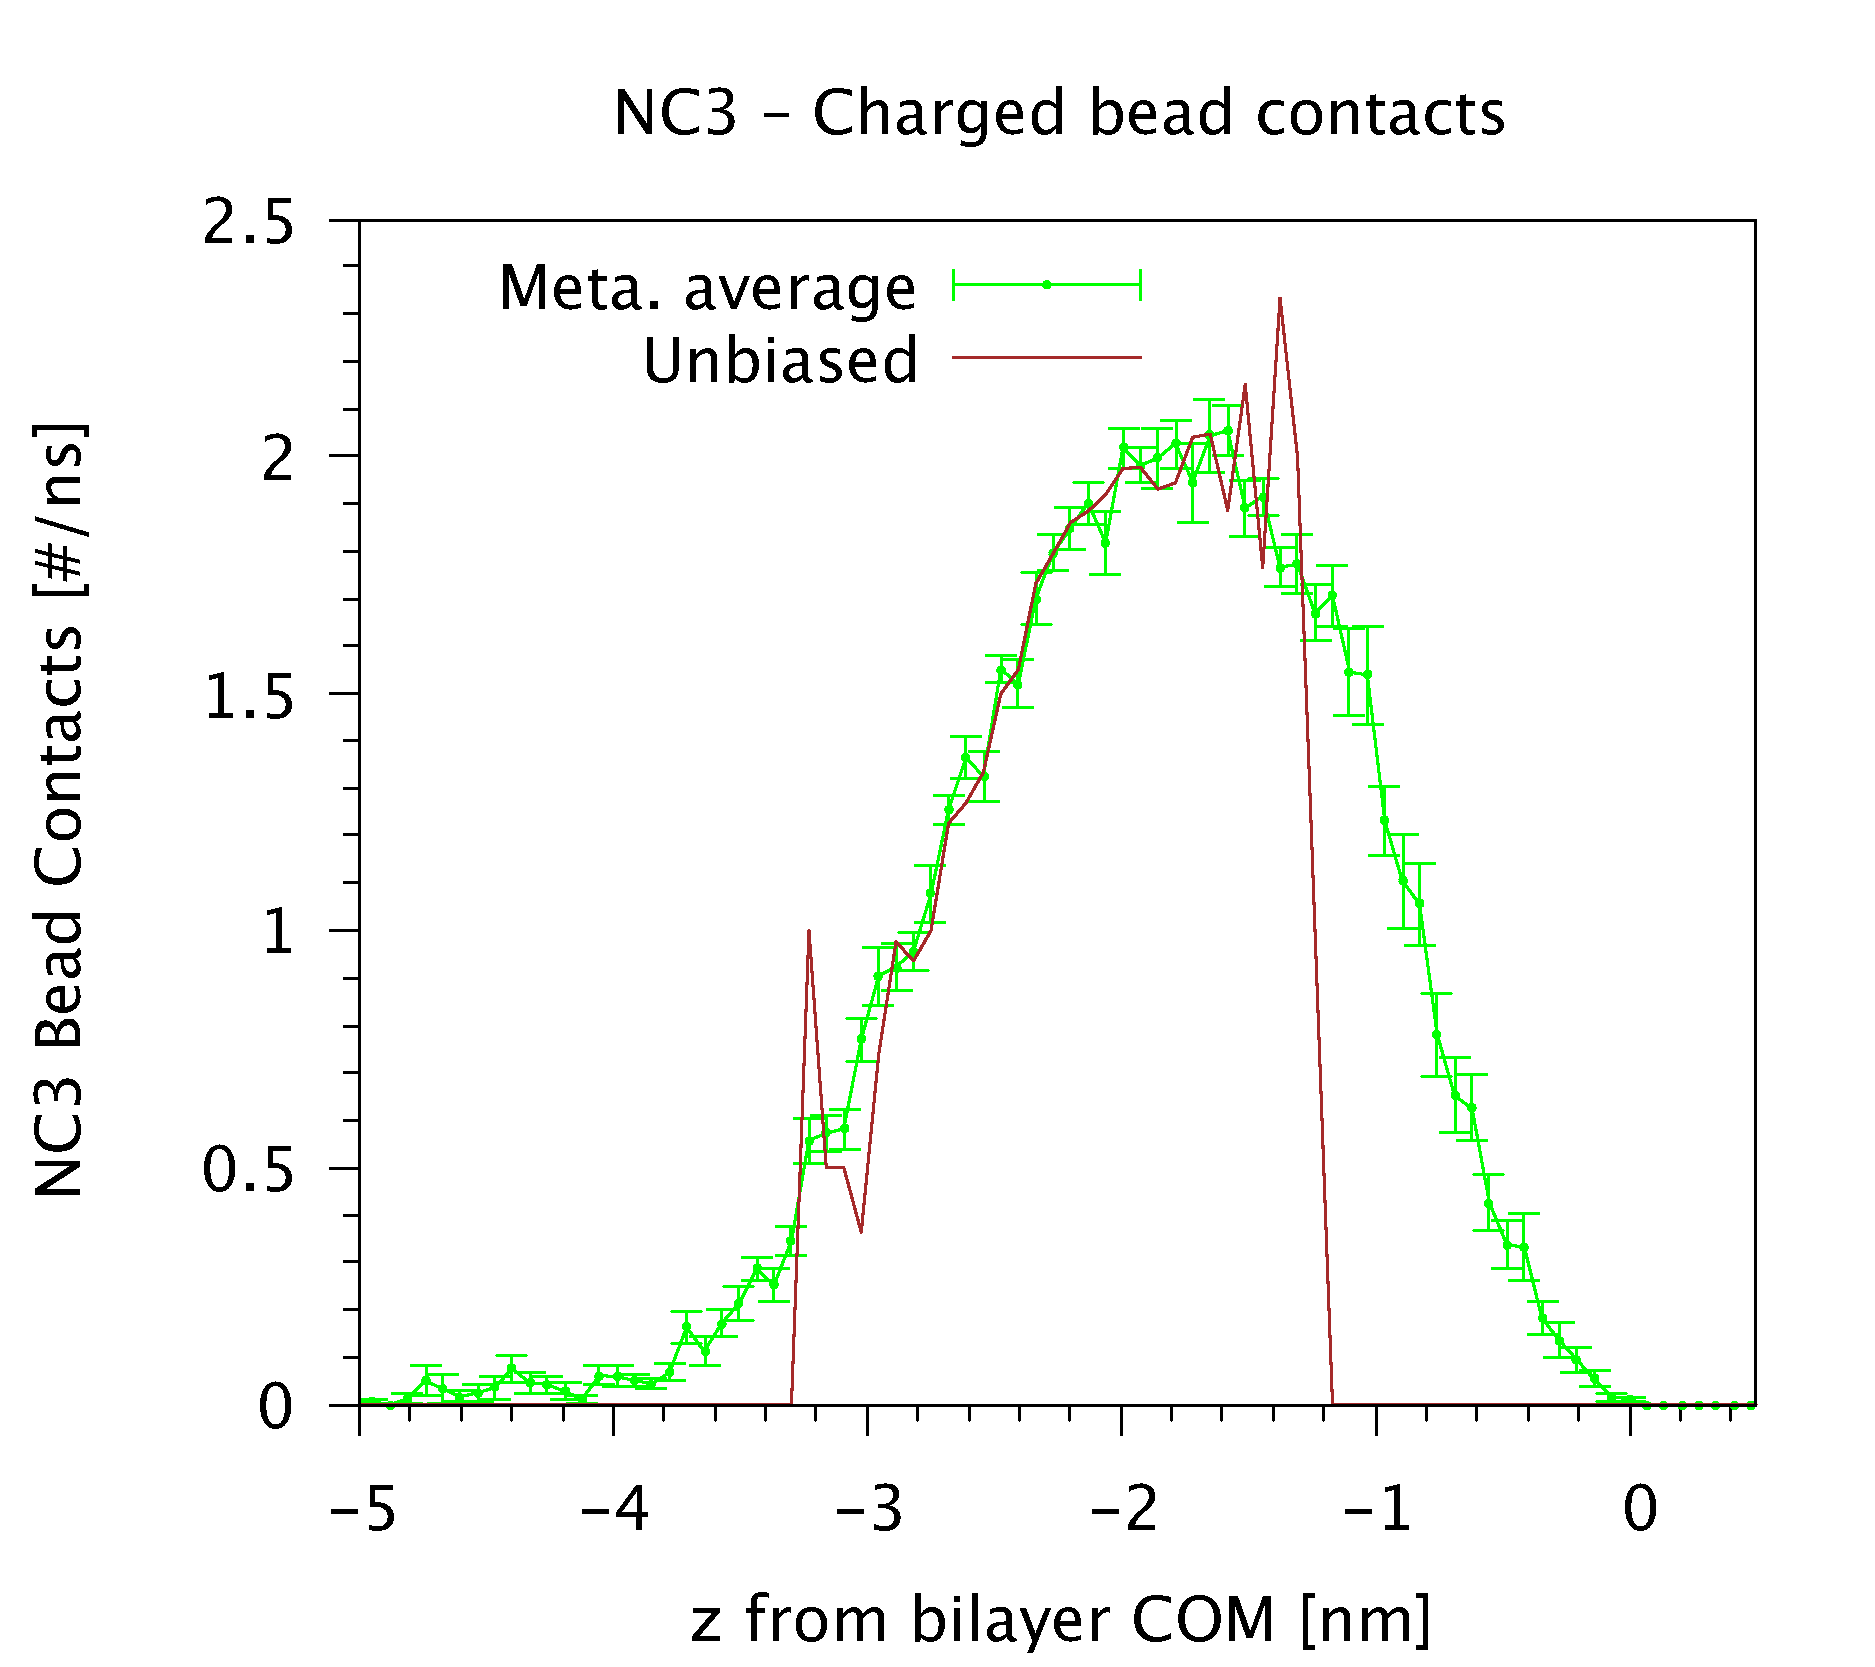
\includegraphics[width=0.5\textwidth]{./img/results/patchedNC3Contact}
	}
	\caption{(a-b) Number of contacts per ns between the \acs{PW} beads and the charged bead in function of the $z$ distance of the charged bead from the bilayer \acs{COM} for the striped \acs{NP} (a) and the random one (b). (c-d) The same for the coline group and the charged bead for the striped \ac{NP} and the random one (d). For each plots the number of contacts are in comparison with the corresponding unbiased runs.}
\end{figure}
\restoregeometry


\section{NP and membrane properties}
%Proprietà generali
%Coef di diffusione stato ancorato, stato idrofobico

\begin{table}[h!t]
	\centering
	\begin{tabular}{lccc}
		\toprule
		\,		 & striped($1$:$1$)		& random($1$:$1$)		& random($1$:$2$)					\\ \toprule
		$D^h_{\text{NP}}$ [$10^{-8}$~cm$^2$/s] & $12 \pm 2$ & $5 \pm 2$ & $5.7 \pm 0.7$ 				\\ \midrule
		$D_{tl}$ [$10^{-8}$~cm$^2$/s] & $30 \pm 1$ & $\mathbf{25 \pm 1}$ & $\mathbf{27.8 \pm 0.1}$	\\ \midrule
		$D_{bl}$ [$10^{-8}$~cm$^2$/s] & $\mathbf{22 \pm 2}$ & $27 \pm 3$	& $35 \pm 1$			\\ \midrule
		$\overline{d_z}$ [nm] & $1.996 \pm 0.0016$	& $2.2794 \pm 0.0017$	& $2.7284 \pm 0.0014$	\\ \bottomrule
	\end{tabular}
	\caption{Lateral diffusion coefficients: of the \acs{NP} in the hydrophobic state ($D^h_\text{NP}$), of the lipids in the top leaflet ($D_{tl}$) and in the bottom leaflet ($D_{bl}$). $\overline{d_z}$ is the average $z$ component of the distance between the \acs{COM} of the \acs{NP} and the \acs{COM} of the \acs{POPC} bilayer. The values in bold font refer to the entrance leaflet. Data obtained from my unbiased runs.}
	\label{tab:NPMembProperties}
\end{table}


\section{Structural properties of the bilayer}
%Risucchio delle membrane al recrossing
%Deformazione del leaflet di ancoraggio: RDF e densitymap 2D